\documentclass[a4paper,fleqn,usenatbib]{mnras}  
\usepackage{newtxtext,newtxmath}
\usepackage[T1]{fontenc}
\usepackage{ae,aecompl}
%\usepackage{graphicx}	% Including figure files
\usepackage{amsmath}	% Advanced maths commands
\usepackage{amssymb}	% Extra maths symbols
\usepackage[english]{babel}
\usepackage[dvipdfmx]{graphicx}
\usepackage{parskip}
%\usepackage[export]{adjustbox}
\pdfminorversion 4

%
\usepackage{subfig}
\usepackage{caption}
%\usepackage{subcaption}
%%%%%%%%%%%%%%%%%%%%%%%%%%%%%%%%%%%%%%%%
%\usepackage{txfonts}
%%%%%%%%%%%%%%%%%%%%%%%%%%%%%%%%%%%%%%%%
%\usepackage[options]{hyperref}
% To add links in your PDF file, use the package "hyperref"
% with options according to your LaTeX or PDFLaTeX drivers.
\usepackage{pseudocode}
%
% Enable mutiple title row on tables.
\usepackage{multirow,booktabs}
%%%%%%%%%%%
% 
% Dealing with ``too many unprocessed floats'' use it with \clearpage 
\usepackage[section] {placeins}

% Defining inentation
\newcommand{\defindent}{\setlength{\parindent}{4ex}}
\newcommand{\zeroindent}{\setlength{\parindent}{0ex}}

% For marginal notes
%\usepackage{marginnote}
%\usepackage{booktabs}

\title[Estimating the atmospheric parameters of M-type
  stars]{Estimates of the atmospheric parameters of M-type stars: a
  machine learning perspective.}

\author[L. M. Sarro et al.]
          {
L.M. Sarro$^{1}$\thanks{lsb@dia.uned.es},
J. Ordieres-Mer\'e$^{2}$,       
A. Bello-Garc\'ia$^{3}$, 
A. Gonz\'alez-Marcos$^{4}$, 
E. Solano$^{5}$
\\
$^{1}$Department of Artificial Intelligence,Universidad Nacional de Educaci\'{o}n a Distancia, c/ Juan del Rosal, 16, 28040 Madrid.\\
$^{2}$Universidad Polit\'{e}cnica de Madrid (UPM), ETSII. PMQ Research Group, Jos\'{e} Guti\'{e}rrez Abascal 2, 28006 Madrid, Spain. \\
$^{3}$Universidad de Oviedo, Construction and Manufacturing Engineering Department, Campus de Viesques s/n, Gij\'{o}n, Asturias, Spain. \\
$^{4}$Universidad de la Rioja, P2ML Research Group, San Jos\'{e} de Calasanz 31, 26004 Logro\~{n}o, La Rioja, Spain. \\
$^{5}$Centro de Astrobiolog\'{\i}a (CSIC-INTA), Ctra. Ajalvir km 4, E-28850 Torrejón de Ardoz, Madrid, Spain.\\
}
\date{Accepted XXX. Received YYY; in original form ZZZ}

% Enter the current year, for the copyright statements etc.
\pubyear{2017}

\begin{document} 
\label{firstpage}
\pagerange{\pageref{firstpage}--\pageref{lastpage}}
\maketitle

\begin{abstract}
    Estimating atmospheric parameters of M type stars has been a
    difficult task due to the lack of simple diagnostics in the
    stellar spectra.  We aim at uncovering good sets of predictive
    features of the stellar atmospheric parameters ($T_{\rm eff}$,
    $\log(g)$, [$M/H$]) in spectra of M type stars. We define two types
    of potential features (equivalent widths and integrated flux
    ratios) able to explain the atmospheric physical parameters. We
    search the space of feature sets using a Genetic Algorithm that
    evaluates solutions by their prediction performance in the
    framework of the BT-Settl library of stellar spectra. Thereafter,
    we construct eight regression models using different machine
    learning techniques and compare their performances with those
    obtained using the classical $\chi^2$ approach and Independent
    Component Analysis (ICA) coefficients. Finally, we validate the
    various alternatives using two sets of real spectra from the IRTF
    and Dwarf Archive collections (DA).  We find that the cross-validation
    errors are poor measures of the performance of regression models
    in the context of physical parameter prediction in M type
    stars. For R$\sim$2000 spectra of the signal-to-noise ratios
    typical of the IRTF and DA, feature
    selection with Genetic Algorithms (GA) or alternative techniques
    produces only marginal advantages with respect to representation
    spaces that are unconstrained in wavelength (full spectrum or
    ICA). We make available the atmospheric parameters for the two
    collections of observed spectra sd online material.
    
\end{abstract}


\begin{keywords}
Methods: data analysis; Methods: statistical;
     Techniques: spectroscopic; Stars: atmospheres; Stars: fundamental
     parameters; Stars: late-type; Stars: statistics;
\end{keywords}

%

\defindent{}

\section{Introduction}
\label{sec:intro}

% The importance of M stars

% The problem of estimation of stellar parameters in the M regime: bands, no con
tinuum...
% who and what. Teff calibrations
% \cite{rajpurohit}
% \cite{amelia}

% Atlases 
%\cite{2013arXiv1306.3709B} % for lambda > 1.1 um :(
%\cite{2009ApJS..185..289R} %IRTF library of cool star

%\cite{2012ApJ...748...93R} % Metall. and Teff indicators in the K band! :(

% Summary of spectral diagnostics in the IR for M stars

% Outline of the paper

In this work we explore the possibility to define spectral features
for the automated inference of the atmospheric parameters of M type
stars using Machine Learning techniques. In Section \ref{sec:meth} we
describe the methodology used to define and evaluate the spectral
features; in Section \ref{sec:irtf} we apply the methodology described
in Section \ref{sec:meth} in the context of the wavelength coverage
and resolution of the IRTF collection of spectra; we describe the
feature definition results and evaluate them for the task of
predicting physical parameters on the actual observed spectra that
make up the collection. Section \ref{sec:ipac} describes the same
steps in the context of the IPAC collection of spectra. Finally,
Section \ref{sec:summary} summarises the main results and conclusions
of the paper.


\section{Methodology.}
\label{sec:meth}
The objective addressed in this Section is to develop an automated
procedure to identify spectral bands that yield good atmospheric
temperature, gravity and metallicity (hereafter physical parameters)
diagnostics for M type stars. Given the lack of a calibration set of
benchmark stars with observed spectra and homogeneous coverage of the
space of physical parameters, we must turn to synthetic libraries of
spectra. Furthermore, only temperatures and gravities can be
calibrated independently of the spectra \citep[for example as
in][using interferometry]{2003A&A...397L...5S}: all metallicity
estimates in the literature are based on collections of synthetic
spectra, and therefore spectral synthesis codes are the only resource
to construct regression models. Even in the case of interferometry,
the estimates of radii (and therefore gravity) depend on stellar
models (although less strongly) via the limb darkening corrections.

As an alternative to the methods based on genetic algorithms used in
this work, the atomic or molecular line/band parameters can be used in
principle to select the spectral features that are more sensitive to
changes in the physical parameters as
in \cite{2016A&A...587A..19P}. However, the suitability of spectral
features as diagnostics of the stellar atmospheric properties depends
not only on the individual behaviour of each line/band, but also on
the relative properties of neighbouring features in the same spectral
region, that may overlap depending on the spectral
resolution. Furthermore, good spectral diagnostics at a given
signal-to-noise ratio (SNR) may show a severely degraded predictive
power in the low SNR regime. Therefore, we propose an alternative
selection approach that takes the resolution and SNR ratio into
account, to assess the utility of spectral features for the task of
inferring physical atmospheric parameters. 

In the following, we adopt the BT-Settl library of synthetic spectra
(\cite{2013MSAIS..24..128A}) as the framework where spectral
diagnostics will be searched for. These synthetic spectra were
pre-processed in several steps as described below.

\subsection{Spectral preprocessing}

First, and in order to define good temperature diagnostics, spectra
between 2000 and 4200K in steps of 100 K were selected, with $\log(g)$
in the range between 4 and 6 dex (when g is expressed in cm/s$^{-2}$),
in steps of 0.5 dex. The metallicity of the representative spectra was
restricted to the set 0, 0.5 and -1 dex.  This yields a total set size
of 535 available spectra.

A series of preprocessing steps were then carried out in order to
match the spectral resolution and wavelength coverage and sampling of
the synthetic library to that of the collection of observed spectra
(IPAC or IRTF, see below). This required the definition of a common
wavelength range present in all available observed spectra, and the
subsequent trimming to match that range. A unique wavelength sampling
was also defined and all spectra (synthetic and observed) interpolated
to match the sampling. Finally, all spectra, both synthetic and
observed were divided by the integrated flux in order to factor out
the stellar distance.

In order to avoid selecting spectral features that are good predictors
only in the unrealistic SNR=$\infty$ regime, the search for optimal
diagnostics of the atmopheric parameters of M stars was carried out
for three SNR values (10, 50 and $\infty$) by degrading the synthetic
spectra with Gaussian noise of zero mean. These values were found to
be sufficient in a wide range of experiments carried out in parallel
and described in \cite{}. The special SNR=$\infty$ case has been
retained for the sake of completeness although \cite{} show that
training sets derived from noiseless spectra are, at best,
unnecessary, and at worst damage performance severely. 

\subsection{Feature definition and selection}
\label{subsec:FD}

As mentioned in Sect. \ref{sec:intro}, defining good spectral
diagnostics for the prediction of atmospheric physical parameters of M
stars is an extremely difficult task .

The work in \cite{cesetti} defined wavelength regions in the I and K
bands optimal for the diagnostic of physical parameters based on the
sensitivity exhibited by the flux emitted in these segments to changes
of the physical parameters. The sensitivity was measured in terms of
the derivative of the flux with respect to the physical parameter. The
approach adopted here is to select spectral features that yield the
best accuracy when used as predictive variables in a regression model
that estimates the stellar atmospheric physical parameters ($T_{eff}$,
$\log(g)$ and metallicity). The evaluation of the accuracy of the
estimates produced from a subset of features is described further
below. We consider the effective temperature as the dominant parameter
influencing changes in the stellar spectra (a strong feature) and
thus, it was estimated first, and then used as input in the regression
models for the gravity and metalicity.

Here, a feature $F$ is defined as

\begin{equation}\label{eq:featureDefinition}
  F = \int_{\lambda_{1}}^{\lambda_{2}} (1-\frac{f(\lambda)}{F_{cont}} \cdot {\rm d}{\lambda})
\label{eq:featuredef}
\end{equation}

where $f(\lambda)$ denotes the normalized flux from the star at
wavelength $\lambda$, and where $F_{cont}$ is the average flux in a
spectral band between $\lambda_{cont;1}$ and $\lambda_{cont;2}$. We
explain below how we search for the band definitions that produce
physical parameter predictions with the smallest errors.

Another type of features defined as

\begin{equation}\label{eq:feature2}
  F' = \frac{ \int_{\lambda_{1}}^{\lambda_{2}}f(\lambda) \cdot {\rm d}{\lambda}}
               {\int_{\lambda_{3}}^{\lambda_{4}} f(\lambda) \cdot {\rm d}{\lambda}} 
\end{equation}

were considered, where $\lambda_1, \lambda_2, \lambda_3$, and
$\lambda_4$ delimit two spectral bands such that the ratio of the
integrated fluxes in the two bands is hoped to be a good predictor
(alone or in combination with other features) of the star atmospheric
physical parameters. The results obtained with this alternative
feature definition did not differ significantly on average from the
ones observed with the one adopted in Eq. \ref{eq:featureDefinition},
and including them here would result in an excessively lengthy
paper. In view of the equivalent global performances, we preferred the
former because it allows direct comparison with the features proposed
by \cite{cesetti}.

We used Genetic Algorithms (hereafter GAs) to solve the optimization
problem described above, that is, the problem of finding the features
(band boundaries) that minimize the prediction error of a regression
estimate of the physical parameters. We used the implementation of
genetic algorithms publicly available as the R \citep{R2013} GA
package. The concept of using in-silico evolution for the solution of
optimization problems was introduced
by \cite{holland1975adaptation}. Although its application is now
reasonably widespread \citep[see e.g. ]{goldberg1989genetic}), they
became very popular only when sufficiently powerful computers became
available. GAs were presented to the astronomical community
in \cite{1995ApJS..101..309C}, and have been used extensively in the
past \citep[see][for the last application of GAs in astronomy at the
time of writing]{}.

For the sake of simplicity let us define Genetic Algorithms (GAs) as
search algorithms that are based on the principle of evolution by
natural selection. The procedure works by evolving in the sense
explained below, chromosomes (in our case, sets of spectral features
as defined by Eq. \ref{eq:featuredef}) from an initial random
population. Evolution proceeds via cycles of differential replication,
recombination and mutation of the fittest chromosomes. The concept of
fittest is context dependent, but in our case fitness is defined in
relation with the accuracy with which a given chromosome (a set
$\{F_i\}$ of spectral features) predicts the physical parameters.

The data set used to search for the optimal set of spectral features
will be, as mentioned before, the BT Settl collection of synthetic
spectra, where each spectrum is tagged with the effective temperature,
gravity and metallicity of the model atmosphere from which the
spectrum emerged.

The implementation of the GA comprises the following steps:

\begin{itemize}
\item \textbf{Stage 1}:{Definition of the population of
potential features (chromosomes).}

\item \textbf{Stage 2}:{Each chromosome in the population
is evaluated by its ability to predict the physical parameters of each
star in the dataset (fitness function). }

\item \textbf{Stage 3}:{Stage 3: Chromosome selection. The new
generation of individuals is initialised by tranferring a number of
the most fitted ones in the previous generation. The percentage of
individuals transferred is known as the degree of elitism. }

\item \textbf{Stage 4}:{The population of chromosomes is replicated. 
 Chromosomes with higher fitness scores will generate more numerous
 offspring.}

\item \textbf{Stage 5}:{The genetic information contained in
the replicated parent chromosomes is combined through genetic
crossover. Two randomly selected parent chromosomes are used to create
two new chromosomes.}

\item \textbf{Stage 6}:{Mutations are then introduced in the
chromosome randomly. These mutations produce new genes used in
chromosomes.  Steps 5 and 6 are applied over the chromosomes
established at Step 4.}

\item \textbf{Stage 7}:{This process is repeated from Stage 2 until 
a target accuracy is achieved or the maximum number of iterations is
attained.}

\end{itemize}

We test features defined by bands (the numerator and denominator of
Eq. \ref{eq:featureDefinition}) that comprise ten consecutive bins
(fluxes) of a spectrum. The bands tested in different features may
overlap by as much as 5 consecutive bins (which in practice implies
that we define the first feature as the spectral chunk between
wavelength bins $i=1$ and $i=10$, the second feature between bins
$i=6$ and $i=15$, the third feature between bins $i=11$ and $i=20$,
etc). The spectral bands in the numerator and denominator of a test
feature cannot overlap.

It would be possible to evaluate the predictive performance of
individual features defined with Eq. \ref{eq:featuredef}. An obvious
conceptual limitation of this univariate approach (considering
chromosomes that code a single predictive feature) would be the lack
of consideration that features work in the context of interconnected
pathways and, therefore, it is their behavior as a group that has to
be evaluated in terms of the predictive accuracy. In other words, a
single feature can yield a poor predictive performance alone, but
improve very significantly the predicton accuracy when used in
combination with other features. Multivariate selection methods thus
seem more suitable for the analysis of the regressors since variables
are tested in combination to identify interactions between
features. In this work we define a chromosome as a set of ten
individual genes, and each gene codes a pair of non-overlapping
spectral bands, the ratio of which is used as predictor of the
physical parameters according to (\ref{eq:featureDefinition}).

The population size was set to 8000 individuals and the maximum number
of accepted iterations set to 4000. We produced three randomly started
populations so as to provide enough initial variety. The crossover and
mutation probabilities were set to 0.85 and 0.35 respectively. Elitism
was fixed to 0.15. We used a binary codification of the chromosomes
and a parallel implementation of the GA in a farm of fifteen computers
per physical parameter \footnote{All computations needed for this work
were carried out in the CeSViMa (http://www.cesvima.upm.es/) power7
HPC which involves processors with 8 cores and four threads per core,
running at 3,3 GHz and with 32Gb of RAM each.

Feature fitness was defined in terms of the Akaike Information
Criterion (AIC) for linearity between the potential feature against
the physical parameter.{bf TODO: RMSE? Why AIC?}  

It is important to stress that the regression model used to evaluate
the fitness of the feature sets (chromosomes) is not the same model
that will be used in practice to predict physical parameters for
observed spectra as described in Section \ref{ssub:models} below. For
fitness evaluation in the GA we used a simple multilinear model for
the sake of speed, given the extreme size of the search space of all
possible combinations of 10 spectral features. In the IRTF context,
these 10 features in each chromosome are selected amongst the roughly
6000 potential features. This is $\binom{6000}{10}$ which has an order
of magnitude of $10^{24}$. 

The GA procedure provides us with a large collection of chromosomes,
each one of them consisting of ten spectral features.  Although these
are all potential solutions of the problem, it is not immediately
clear which one should be selected for the final regression model. In
this work we have selected the most frequent features amongst the
fittest chromosomes as predictive variables of the physical parameters
in regression models. Features appearing in less than five chromosomes
were initially discarded as they can not be relevant by themselves and
just arise randomly by combination with other stronger chromosomes.

{\bf TODO: Rewrite} It is relevant to say that when genes of a
chromosome induced as ratio of two gaussian variables have extremely
wide wings if any of the features is centered around zero, the fitness
criteria removes it as a cadidate feature as it is not able to explain
the physical parameter.  Therefore, the single regression model
should, to some extent, be descriptive of the population. The simpler
strategy would be to use the frequency of the chromosome in the
population as criterion for inclusion in a forward selection
strategy. However we prefered to select the features based on their
highest fitness as it enhances the value of the direct contribution to
explain the physical parameter.  As we have accepted that compex
interactions between individual features are possible, it was selected
a fixed number of features allowing both, enough room for developping
those complex dependency relationships but to keep the complexity of
the comming regression models under control.  Therefore, it was
selected ten as the suitable number of features being considered per
physical parameter.

Once the GA has generated a proposal set of features for predicting
each of the physical parameters, the next step consists in training
the regression model based on these features. This is described in the
nest Section.

\subsection{Models considered.}
\label {ssub:models}

Once a feature set (the predictor variables) was selected from the
output of the GA, we construct regression models to predict the
physical parameters (response or predicted variables) from it. In the
context of Machine Learning, constructing a regression model consists
in using a training set (a set of cases defined by the predictor
variables for which the predicted variables are available) to infer
the parameters of an (often analytical) mapping between predictor and
predicted variables. The regression model parameters should not be
confused with the physical parameters of the atmosphere we aim at
inferring. {\bf TODO: Check if every occurrence of parameter is clear}

In this case, our training set is again the BT Settl collection of
synthetic spectra, for which we already computed the predictor
variables (the features) as part of the GA selection procedure. And,
of course, for each spectrum we also have available the effective
temperature, the gravity and the metallicity. Once the model is
trained, we will apply it to observed spectra as described in
Sections \ref{sec:irtf} and \ref{sec:ipac}.  

Several regression models are trained for the prediction of each
physical parameter in order to evaluate their performance:

\begin{itemize}

\item {Bagging with Multiadaptive Spline Regression Models \emph{(hereafter MARS)}.}

\item {Random Forest Regression Models \emph{(RF)}.}

\item {$k$-Nearest Neighbours \emph{(KNN)}.}

\item {Generalized Boosted Regression Models \emph{(GBM)}.}

\item {Support Vector Regression with Gaussian Kernel \emph{(SVR)}.}

\item {Multi-layer Perceptron Neural Networks \emph{(NNET)}.}

\item {Kernel Partial Least Squares Regression \emph{(KPLS)}.}

\item {Rule Regression Models \emph{(RR)}.}

\end{itemize}

In order to assess the validity of our feature sets we also compare
the predictions based on them with other input spaces. In particular,
we also compute physical parameters that yield the the minimum
$\chi^2$, and train a Projection Pursuit regression models with the
Independent Components derived from each spectrum. {\bf TODO: add
reference for ICA}.

Including here a sufficient description of each and every regression
model that we trained would render the manuscript excessively lengthy
but interested readers can find additional information in
\cite{baraud2002model,geman1992neural,elith2008working,meyer2003support,svetnik2003random}. Suffice it to say that each one of them can be thought of as
a parametric model that predicts one physical parameter from an input
vector. The input vector can be the full normalised spectrum, the ICA
lower-dimensional representation of the full spectrum, the spectral
features selected by \cite{cesetti} or those selected by the GA. The
regression model parameters are infered (using strategies that differ
from one regression model to the other) from a set of examples. As
explained above, this set of examples (spectra of stars for which we
know the physical parameters) is called the training set, and the
process by which the model parameters are determined from the training
set, is called training of the model. In the next paragraph we give
minimal details of each regression model trained, and references for
the interested reader.

In order to avoid the well known problem of overfitting \cite[see
e.g.][]{Dietterich:1995:OUM:212094.212114}, we use five-fold
cross-validation to estimate the prediction errors. $n$-fold cross
validation consists in dividing the trainins set into $n$ disjoint
subsets and training ten different regression models, each one of them
with ($n$-1) of the $n$ subsets. The $n$-th subset not used for
training is used to estimate the errors.

As every type of model has its own set of tunable parameters as well
as its own training procedure, the authors have selected a common
R \cite{R2016} wrapper for all models named caret (short for
Classification And REgression Training) \cite{caret}.  This wrapper
enables a common interface, as well as the use of the same set of
training/set samples for the adopted five-fold cross-validation error
estimation. As explained above, each regression model has its own set
of model parameters. For each model we have searched for the parameter
set that minimized the Root Mean Square Error (RMSE) in a grid of
values defined {\it ad hoc} for each technique.

The adopted procedure for learning the models can then be summarized
as the pseudocode \ref{caretp}.

{\bf TODO [Joaquín]: define each element in the pseudocode}

\begin{pseudocode}[shadowbox]{Model Learning}{DataSet,ParRanges}
\label{caretp}
 \mathcal{S}_{ModelParameters} \GETS ParRanges \\
 \mathcal{S}_{DataFolders} \GETS Preprocess(DataSet) \\ 
 \FOREACH x \in \mathcal{S}_{ModelParameters} \DO
  \BEGIN
    \FOREACH z \in \mathcal{S}_{DataFolders} \DO
      \BEGIN
	HDS(z) \GETS \mbox{Hold-out specific samples} \\
	Model(z) \GETS Fits(\mathcal{S}_{DataFolders} \setminus HDS(z) ) \\
	Perf(z) \GETS Predicts(Model(z),HDS(z)) \\
      \END \\
    Perf(x) \GETS Average(Perf(z)) \quad \forall z \in \mathcal{S}_{DataFolders} \\
  \END \\
  
  OPS \GETS argmax(Perf(y)) \quad \forall y \in \mathcal{S}_{Modelparameters} \\
  Model \GETS Fits(DataSet, OPS) \\
\end{pseudocode}

As mentioned above, the training set was constructed from the BT Settl
library of stellar spectra. The interested reader may find different
approaches in the literature to the problem of finding an optimal set
of training examples. \cite{hoggCannon} for example prefer to use real
observed spectra rather than synthetic libraries to create a
generative model in which the individual spectral fluxes are modelled
as second degree polynomials with the physical parameters as
arguments. The real observed spectra have physical parameters taken
from the literature, which in turn are almost always inferred using
synthetic spectral libraries. In our opinion, this approach does not
solve the dependence of the predicted parameters on the necessarily
imperfect synthetic libraries, but has the advantage that the relative
frequencies of examples in the training set represents better the
biases naturally encountered in surveys than the uniform sampling of
parameter space found in synthetic libraries. Recently, \cite{heiter}
have started a program to compile a set of stars with accurate
physical parameter determinations infered independently of
spectroscopic measurements and atmospheric models (as much as
possible). Unfortunately, this ambitious program only contains 34
stars of spectral types F, G, and K. In the M regime we find similar
approaches in \cite{2014AJ....147...47B} and references therein, where
the atmospheric parameters are derived using interferometric
measurements of stellar radii. Again, this only amounts to a very
small number (21 K and M stars) of examples and a very sparse sampling
of the parameters space.

All efforts to compile training sets of stars with accurate,
homogeneous, and reliable physical parameters derived independently of
spectroscopic measurements are valuable not only because they allow
for the improvement of the stellar atmospheric models but also because
they help increase the reliability of the regression models by making
them independent of these atmospheric models. But until these training
sets with sufficient and homogeneous sampling of the parameter space
are available, we must turn to the use of synthetic libraries.

% Additional text

%In order to assess the
%performance of the regression models, we compare their predictions
%with i) values of the physical parameters from the literature (when
%available); ii) the predictions from the popular $minimum \chi^2$
%distance to spectra in the BT-Settl library.
%;
%iii) parameter predictions based on a projection pursuit regression
%model {\bf Is this correct, Joaquín? Somewhere in your first version
%of the paper it was stated that the ICA components were fed to an SVM
%with C=10 and epsilon=0.001 for temperature, and different values for
%logg and metallicity} trained with projections of the BT-Settl spectra
%onto the set of vectors resulting from an Independent Component
%Analysis (ICA); and finally, iv) predictions from a regression model
%trained with the features proposed by \cite{cesetti} (only for the
%IRTF spectra) {\bf Joaquín, aquí necesitamos explicar qué tipo de
%modelo entrenamos con las features de cesetti.}.
%In the case of features proposed by \cite{cesetti}, such ranges were
%directly provided by their paper and the GA based selection of features 
%was, therefore, not needed.

%It is worthy to said that because of the impact on the emission spectrum 
%for all the pohysical parameters are the same, several strategies were 
%implemented to verify to what end using hierarchical knowledge becomes
%helpful to the modelling procedure. Therefore, extensive set of trials 
%have been conducted to derive gravity and metallicity features with and
%without temperature knowledge. Models were trained to determine the impact of
%such temperature hierarchical contribution and it was found that, 
%no matter of the model considered, the features determined plus the 
%estimated star temperature outperform the same model without the 
%temperature knowledge by about 20\% in case of gravity models and 12\%
%in case of metallicity models.
%Based on those results, GA features for gravity and netallicity were 
%reinforced with the estimated star temperature as an additional feature.


\section{Physical parameters of the IRTF collection of spectra.}
\label{sec:irtf}

In the following, we will summarise the results obtained for the IRTF
data set. We deal with the different physical parameters in separate
Sections. We start by reporting the Root Mean/Median Square Errors
(RMSE/RMDSE) with respect to the parameters gathered from the
literature by \cite{cesetti} and included in their Table 3.

\subsection{Spectral bands selected}
% Rework the sentence  JOM
\textbf{
The GAs were applied to the selection of features for the
prediction of effective temperature from both, noiseless and noisy spectra.
For the IRTF wavelength range and resolution, results in the features have been included
in Table~\ref{tab:irtf-teff-noisy}. 
}
% End of update
Features are ordered by the
fitness value (according to the AIC criterion, as explained in Eq.~\ref{eq:AIC}) and 
we only consider features that are present in at least 5 sets.

% When noise is added to the BT-Settl spectra, we obtain the features
% included in Table \ref{tab:irtf-teff-noisy}.

Table % \ref{tab:irtf-teff-noiseless} and 
\ref{tab:irtf-teff-noisy}
show a very wide variety of features with very few repetitions. Only
spectral features 4, 5, 6, and 9 in the SNR=50 experiment are found
too in the SNR=$\infty$ and SNR=10 feature sets (albeit with different
continuum definitions). This reinforces the impression that the
information useful for the estimation of the effective temperatures is
spread over the entire IRTF spectrum.
% Removing Table A3 => JOM
\textbf{
As a reference, it is used the Table~3 defined in \cite{cesetti}, which
%~\ref{tab:irtf-cesetti} 
lists the features found using sensitivity maps.
}
% End of changes

\begin{figure*}
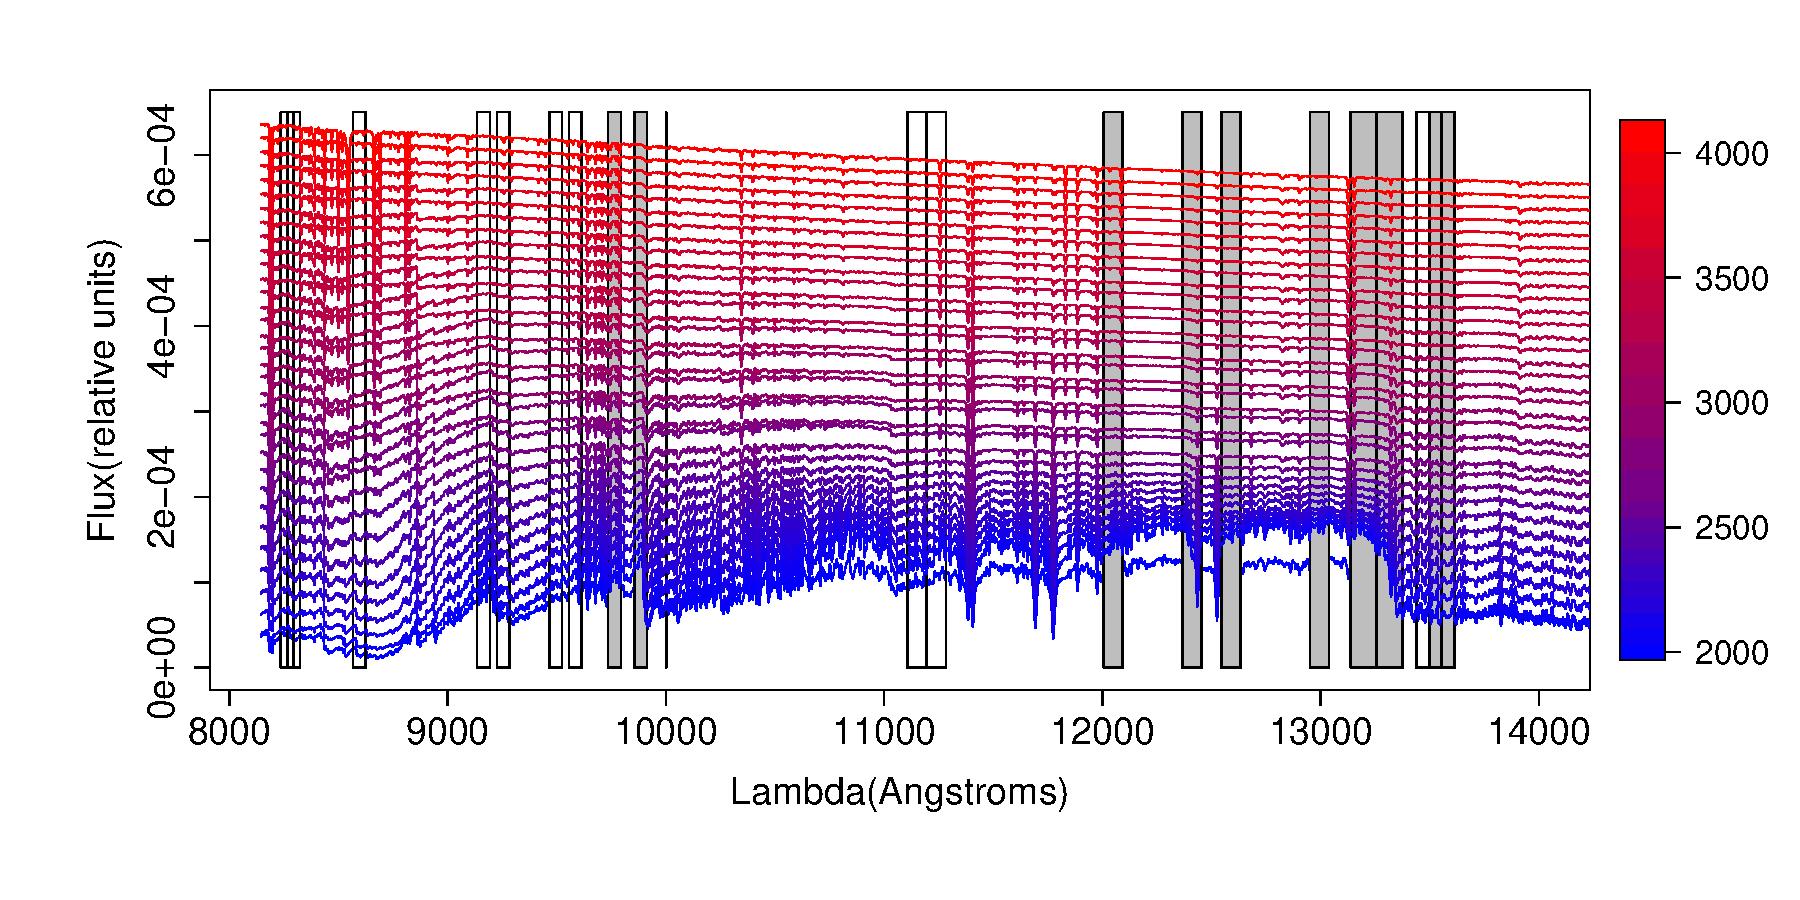
\includegraphics[width=\textwidth]{figs/BT-spectraAtIRTF-Inf-teff2}
 \caption{Features selected by the GA for predicting $T_{eff}$ using
    noiseless BT\_Settl synthetic spectra in the IRTF wavelength range
    and resolution. The BT\ Settl spectra are plot in a colour scale
    that ranges from blue (2000 K) to red (4100 K). The empty boxes
    correspond to the selected features and the grey boxes to the
    continuum bands.}  \label{fig:IRTF-teff}
\end{figure*}

For gravity estimation (on a logarithmic scale), the GA search
procedure produces the features presented in
Table % \ref{tab:irtf-logg-noiseless} and 
\ref{tab:irtf-logg-noisy} for
the noiseless signal and signal-to-noise ratios of 10 and 50,
respectively. In a similar way, the best features found 
by the GA for metallicity estimation are listed in % Table~\ref{tab:irtf-met-noiseless} for the noiseless BT-Settl
% spectra, and in 
Table~\ref{tab:irtf-met-noisy} for signal-to-noise
ratios equal to $ \infty, 10 $ and $ 50 $.

Figures \ref{fig:IRTF-teff}-\ref{fig:IRTF-met} show
graphically the band limits listed in
Tables~\ref{tab:irtf-teff-noisy} to \ref{tab:irtf-met-noisy}
% --\ref{tab:irtf-met-noiseless} 
on a collection of spectra from the BT-Settl library.


\subsection{Regression models}

\subsubsection{Effective temperature models}
\label{sect:irtf-teff}

Table \ref{tab:irtf-teff-rmse} summarises the RMSE/RMDSE for the
complete set of models: the minimum $\chi^2$ estimate based on the
full spectrum ($\chi^2$), the projection pursuit regression based on
the ICA components (PPR-ICA) and models trained on the spectral
features proposed by the GA (GA-RF, GA-GBM, GA-SVR, GA-NNET, GA-MARS,
GA-KPLS, GA-RR). For each model, we report the RMSE/RMDSE obtained for
several noise levels of the training sets.  SNR=$\infty$ corresponds
to noiseless spectra. In the GA-cases, models are trained with the
spectral features found by the Genetic Algorithms when applied to
BT-Settl spectra of the corresponding SNR.

Table \ref{tab:irtf-teff-rmse} shows that performance of classifiers
based on the full spectrum (or in a compressed version in the form of
ICA components) and the best classifier based on features derived from
limited spectral bands is equivalent. The Bartlett test shows that the
variances are homogeneous with a Bartlett\textquoteright s K-squared
of 8.5 with 2 degrees of freedom and a p-value of 0.01426. The
Flinger-Killen test shows that homoscedasticity is verified at the
p=0.005886 level. Finally, the F-ANOVA test clearly shows that there
is no significant difference between models. Thus, we conclude that
the quality of features from the two approaches are equivalent in
predictive performance.  The difference between the performances of
the best classifier ($GA-KNN$; best on average over SNR), the minimum
$\chi^2$ classifier, and the $PPR-ICA$ classifiers are not
statistically significant. 
In any case, it is evident that the RMSE is significantly above the grid
spacing in temperature. We interpret the small differences as an
indication that there is as much information spread over the entire
spectrum shape as can be distilled from a few spectral bands.

The comparison with the effective temperatures compiled by
\cite{cesetti} shows, however, some significant differences across
models when evaluated not by the RMSE/RMDSE, but by the average bias
(see Table \ref{tab:irtf-teff-bias}). 

In general, all regression models tend to predict lower effective
temperatures than those in the literature except in the noiseless
scenario. The models trained with noiseless spectra tend to
overestimate $T_{\rm eff}$, suggesting that the optimal SNR is between
SNR=50 and $\infty$. The minimum-$\chi^2$ approach and the GA-KNN
model systematically underestimate $T_{\rm eff}$ for all SNR
regimes. This shared behaviour is not surprising since minimum
$\chi^2$ is a single nearest neighbour method applied in the space of
the entire spectrum as opposed to the space selected features.

We have found in previous studies that, at least for input spaces
constructed from ICA compressions of the spectra, it is not necessary
to adapt the training set SNR to match exactly that of the prediction
set. On the contrary, we find that two regimes are sufficient to
obtain acceptable results. The two regimes are separated at
SNR=10. The model trained with SNR=50 spectra gives close to optimal
results for spectra with SNRs above 10, while below that limit the
same situation holds for the model trained with SNR=10
spectra \cite{2017MNRAS.465.4556G}.

Figure~\ref{fig:irtf-teff} shows the correlation between the $T_{\rm
eff}$ estimates of the best (in the RMDSE sense) regression models and
the effective temperatures in Table 3 of \cite{cesetti}. 

\begin {figure}
 \centering
  \includegraphics[scale=0.4]{figs/irtf-teffs-literature}
  
  \caption{Comparison of the effective temperatures from the
  literature included in \protect\cite{cesetti} and those inferred from the
  KNN module trained with the GA features (black). In orange and blue
  we show the estimates from the minimum $\chi^2$ estimate and from
  the PPR model based on the ICA components, respectively.}

\label{fig:irtf-teff}
\end {figure}

It is worth noting that in the M star regime, there are 63 effective
temperatures available in \cite{cesetti}, and 46 of the 63 were
estimated from the spectral types using the calibrations
of \cite{1996imsa.book.....O}. We have substituted them with a spline
fit to the combined datasets of M dwarfs in \cite{2013A&A...556A..15R}
and \cite{2012ApJ...757..112B} as it removes systematic biases in the
temperatures between 2500 and 3500 K.

It is not evident that the GA-KNN model performs significantly better
than the minimum $\chi^2$ estimate, but in the following we will
retain the former for further analysis. Figure \ref{fig:irtf-teff}
shows that the GA features can be used to estimate effective
temperatures with an accuracy equivalent to that yielded by full
wavelength range spectra of the same resolution.


We have trained the same non linear regression models discussed above
using the features suggested by \cite{cesetti}. The performance of the
models based on these features are included in Table
\ref{tab:irtf-teff-rmse-cesetti}. From the comparison of Tables
\ref{tab:irtf-teff-rmse} and
\ref{tab:irtf-teff-rmse-cesetti} we can draw the following conclusions:

\begin{itemize}

\item The RMSE for SNR=10 and 50 is equivalent for the regression
  models trained on GA features and those recommended
  in \cite{cesetti};

\item However, the RMDSE from \cite{cesetti} is significantly higher
  in the case of the features for all SNR values.

\item In the unrealistic case of noiseless spectra, the features proposed
  by \cite{cesetti} produce RMSE and RMDSE significantly worse than
  the GA features.

\end{itemize}

However, the cross-validation errors are far from informative with
respect to the true performance when the models are applied to real
data. In the case of the features defined by \cite{cesetti}, we find
that the best RMSE/RMDSE (obtained not from cross-validation but from
the comparison with the effective temperatures in Table 3
of\cite{cesetti}) is attained by the CES-NNR
model. Figure \ref{fig:irtf-cesteff} shows the graphical comparison of
the CES-NNR predictions with the Table 3 reference values. Again, and
in the rest of this work, we substitute the effective temperatures in
that Table that were estimated using the \cite{1996imsa.book.....O}
calibration with those from the spline fit described above.

\begin {figure}
 \centering
  \includegraphics[scale=0.4]{figs/irtf-CESteffs-literature}
  
  \caption{Comparison of the effective temperatures from the
  literature included in \protect\cite{cesetti} and those inferred from the
  NNR module trained with the features introduced in \protect\cite{cesetti}
  (black). In orange and blue we show the estimates from the minimum
  $\chi^2$ estimate and from the PPR model based on the ICA
  components, respectively.}

\label{fig:irtf-cesteff}
\end {figure}

Figure \ref{fig:irtf-cesteff} shows that the features found by the GA
are to be prefered to the ones proposed by \cite{cesetti}. 

\subsubsection{Surface gravity models}

For the validation of our models, we only have 10 literature values of
the surface gravity available in Table 3 of
\cite{cesetti}. Unfortunately, this is too small figure to draw
significant conclusions on the comparison of methodologies from
external data. Hence, we are left only with plausibility arguments for
the selection of models. In this Section $\log(T_{\rm
eff})$--$\log(g)$ diagram comparisons will be used to select the most 
plausible model results. 

An important difference with respect to the models discussed
above is that we use the $T_{\rm eff}$ estimated in the previous stage
as input of our models. It introduces an average improvement in the
RMSE/RMDSE of 20\% with respect to the models without input
information on the effective temperature although it represents a risk
if the $T_{\rm eff}$ estimate is in gross error.

Table~\ref{tab:irtf-logg-rmse} shows the RMSE and RMDSE of the
cross-validation experiments for the $\log(g)$ regression models and
the same SNR regimes discussed for the estimation of $T_{\rm eff}$. We
have assessed the models according to plausibility arguments relative
to the distribution of the model predictions in $T_{\rm
eff}$--$\log(g)$ diagrams.  Figure~\ref{fig:lt_lg_ga} shows this
distribution for four models selected based on these plausibility
criteria: GA-RR, GA-PLS, GA-KNN (the three of them for SNR=50), and
PPR-ICA (clockwise, starting at the top left corner). All four panels
show a tendency towards lower surface gravities at the coolest end,
and a reasonable capability to separate dwarfs from giants, and giants
from supergiants. We include as orange squares the recent predictions
by \cite{esm1} and \cite{esm2} for a set of sources with
high-resolution infrared spectra. The estimates are in reasonable
agreement with the extrapolation of the distributions that can be
guessed from the values in Table 3 of \cite{cesetti} (represented with
black filled symbols). Since we cannot propose quantifications of this
plausibility argument valid for all luminosity classes, we let the
reader decide which estimate (GA-RR, GA-PLS, GA-KNN, or ICA-10) is to
be prefered. If we judge only by the concordance with the locus
defined by the M dwarfs in the studies by \cite{esm1} and \cite{esm2},
then ICA-10 is to be preferred.

\begin{figure*}
 \begin{center}
   \includegraphics[width=\textwidth]{figs/ordieres-fig4}
\caption{$\log(T_{eff})$--$\log(g)$ diagrams produced by the GA-KNN
   (SNR=$\infty$) effective temperatures and gravities derived with
   the GA-RR (SNR=50), GA-PLS (SNR=50), GA-NNR (SNR=50), and
   $PPR-ICA-10$ models (clockwise, starting from the top left
   plot). Squares represent dwarfs stars, triangles represent
   luminosity class {\sc III} and circles represent luminosity classes
   {\sc I} and {\sc II}. Black symbols represent values taken
   from \protect\cite{cesetti}, orange symbols correspond to values
   derived from high-resolution infrared spectra by \protect\cite{esm1}
   and \protect\cite{esm2}, and red symbols are our own predictions.}

\label{fig:lt_lg_ga}
 \end{center}
\end{figure*}

Figure \ref{fig:irtf-ces} shows the equivalent diagram for predictions
obtained from the features selected in \cite{cesetti}. Again, we
select the regression models that yield the most plausible
$\log(T_{\rm eff})-\log(g)$ distributions with no quantitative
criteria defined to select the models. It is again evident the
superiority of the GA-based features over those defined
by \cite{cesetti}.

\subsubsection{Metallicity models} 
\label{sect:irtf-met}

Finally, the same machine learning models are trained to infer the
metallicity, again considering the effective temperature as an input
feature as in the $\log(g)$ regression
models. Table~\ref{tab:irtf-met-rmse} shows the RMSE and RMDSE
obtained for the cross-validation experiments of each regression
model. The minimum cross-validation errors are consistently obtained
with the minimum $\chi^2$, $PPR-ICA$ and $GA-KNN$ (with some
exceptions). The differences from these cross-validation experiments
are only marginal, but we see that even at these intermediate
resolutions the reduction of dimensionality (either with ICA or GA)
produces an improvement in the predictions. 

This is even more evident if we compare our predictions with more
recent metallicity estimates not included in \cite{cesetti}. We have
gathered estimates for stars in both the IRTF collection and a series
of recent metallicity catalogs
by \cite{RA2012}, \cite{NevesIII}, \cite{Newton2014}, \cite{Gaidos2015},
and \cite{Mann2015}. All of the aforementioned references provide us
with estimates of the iron abundance ratio [Fe/H] except \cite{RA2012}
that provides both the overall metallicity [M/H] and the [Fe/H]
ratio. Our estimates, coming from the BT-Settl library, are for the
[M/H] ratios, so some offset could be expected from the different
nature of the quantities compared. Hence, when comparing our estimates
with those from the literature, we compute the RMSE or RMDSE after
subtracting any difference in the mean. It turns out that, after
correcting for these different scales, $PPR-ICA$ trained with SNR=10
examples yields the lowest RMSE/RMDSE. Figure \ref{MIRTF_ICA_10}
represents the estimates of [M/H] obtained from the $PPR-ICA$ based
regressor, as a function of the values taken from these references for
the sources in common. 

The black empty circles represent values
from \cite{cesetti} ; orange filled circles, values
from \cite{NevesIII}; green filled squares, values that the Vizier
catalog entry for Table 8 of
\cite{NevesIII} links to \cite{Jao}. Although we find no evidence
that \cite{Jao} contains estimates of metallicities; cyan and blue
filled squares, are the values of [M/H] and [Fe/H] respectively
in \cite{RA2012}; red filled squares, values from \cite{Mann2015};
yellow filled squares, values from \cite{Newton2014}; and, finally,
black filles squares, values from \cite{Gaidos2015}.

It is remarkable that the minimum $\chi^2$ predictions result in a
50\% increase in the RMDSE with respect to the ICA-10 models and the
best performing GA-based models. Therefore, we advice against its use
in the context of metallicity estimations. 

 \begin{figure}
 \centering
 \includegraphics[width=0.45\textwidth]{figs/irtf-figs/M-ICA10}

\caption{Comparison
  between metallicity estimates from the literature and predictions
  from the PPR-ICA (SNR=10) model.  Black empty circles represent
  values from \protect\cite{cesetti} ; orange filled circles, values
  from \protect\cite{NevesIII}; green filled squares, values that the
  Vizier catalog entry for Table 8 of \protect\cite{NevesIII} links
  to \protect\cite{Jao}, although we find no evidence
  that \protect\cite{Jao} contains estimates of metallicities; cyan
  and blue filled squares, the values of [M/H] and [Fe/H] respectively
  in \protect\cite{RA2012}; red filled squares, values
  from \protect\cite{Mann2015}; yellow filled squares, values
  from \protect\cite{Newton2014}; and, finally, black filles squares, values
  from \protect\cite{Gaidos2015}.}

\label{MIRTF_ICA_10}
\end {figure}

Figure \ref{fig:irtf-teff-logg-met} summarizes the predictions from a
set of selected regression models in $T_{\rm eff}$ (from the
GA-NN-$\infty$ model), $\log(g)$ (from the GA-RR-50 model) and
metallicity (from the PPR-ICA-10 model). Again, plausibility arguments
such as the lower metallicity of the supergiants apparently give
evidence supporting the good performance of our models, but the lack
of extensive good-quality estimates of the physical parameters of the
IRTF collection of stars prevents us from a more quantitative
assessment of the predictions.

 \begin{figure}
 \centering
 \includegraphics[width=0.5\textwidth]{figs/ordieres-fig8}
\caption{Plane of predictions for $T_{\rm eff}$ (from GA-KNN-$\infty$)
and $log(g)$ (from GA-RR-50) with metallicity predictions from
PPR-ICA-10.}
\label{fig:irtf-teff-logg-met}
\end {figure}

The equivalent plot for predictions based on the features defined
by \cite{cesetti} and the RF model trained with SNR=50 spectra is
included as Figure \ref{fig:irtf-ces-met}.




\section{Physical parameters of the DA collection of spectra.}
\label{sec:ipac}

\subsection{Spectral bands selected}

As for the IRTF spectra, the spectral resolution of the BT-Settl
library was degraded to match the average resolution of IPAC spectra
in the Dwarf
Archives\footnote{http://spider.ipac.caltech.edu/staff/davy/ARCHIVE/index.shtml}. {\bf
What is the average resolution?}. Then, the spectra were trimmed to
produce valid segments between *** and *** {\AA}, which is the
spectral range common to all M stars in the archive. Finally, all
spectra were divided by the total integrated flux in this range in
order to factor out the stellar distance.

There is little hope {\it a priori} for reasonable accuracies with
regression models that predict the surface gravity and metallicity
from such wavelength-limited, low/intermediate resolution
spectra. Anyhow, we provide the results obtained applying the same
methodology as in Section \ref{sec:irtf} (and described in
Section \ref{sec:meth}) to show the limitations.

\subsubsection{Spectral features for the estimation of effective temperatures.}

The application of the GA to the selection of features for the
prediction of effective temperature from noiseless spectra within the
IPAC wavelength range and resolution, results in the features included
in Table~\ref{tab:ipac-teff-noiseless}. Features are ordered by the
fitness value (the AIC){\bf and we only consider features that are
present in at least 5 sets}. For the noisy spectra of SNR=10 and 50 we
select the spectral features listed in
Table~\ref{tab:ipac-teff-noisy}.

{\bf TBD by Luis: interpret the features.}

Tables \ref{tab:ipac-logg-noiseless} and \ref{tab:ipac-logg-noisy}
show the spectral features selected by the GA for noiseless BT-Settl
spectra and the same spectra with SNR=10 and 50, respectively.

Finally, the best features found by the GA for the estimation of the
metallicity are listed in Table~\ref{tab:ipac-met-noiseless} for the
noiseless BT-Settl spectra, and in Table~\ref{tab:ipac-met-noisy} for
signal-to-noise ratios equal to 10 and 50.


\subsection{Regression models}

In the following, we will summarise the results obtained for the Dwarf Archives
data set. We deal with the different physical parameters in separate
Sections. We start by reporting the cross validation Root Mean Square
Errors (RMSE) and Root Median Square Error (RMDSE) for the five-fold
cross-validation strategy, and we subsequently discuss the accuracy of
the predictions with respect to literature values where available.

\subsubsection{Effective temperature models}

Table \ref{tab:ipac-teff-rmse} summarises the RMSE/RMDSE for the
complete set of models: the minimum $\chi^2$ estimate based on the
full spectrum ($\chi^2$), the projection pursuit regression based on
the ICA components (PPR-ICA) and some models trained on the spectral
features proposed by the GA (GA-RF, GA-GBM, GA-SVR, GA-NNET, GA-MARS,
GA-KPLS). For each model, we report the RMSE/RMDSE obtained for
several noise levels of the training sets.

Again, as in the IRTF case, we see that the compression of the spectra
results in a clear performance degradation with respect to the
$\chi^2$ minimization technique results. Figure \ref{fig:ipac_teff} shows
a comparison between the effective temperatures derived from a
spectral type calibration ({\it x} axis) and the predictions of the
best regression models ({\it y} axis). In particular, we have
converted the spectral types available in the {\it DwarfArchives.org}
collection to effective temperatures using the same spline fit
described in the IRTF Section. It shows that the best results based on
the ten features selected by the GA are barely equivalent to the
prediction accuracy of the $\chi^2$ estimates. The decrease in
predictive variables results in a simpler and faster model, but the
$\chi^2$ model is already simple so our conclusion is that the feature
selection in this context of low resolution spectra in the optical
range is unnecessary.

\begin {figure*}
\centering 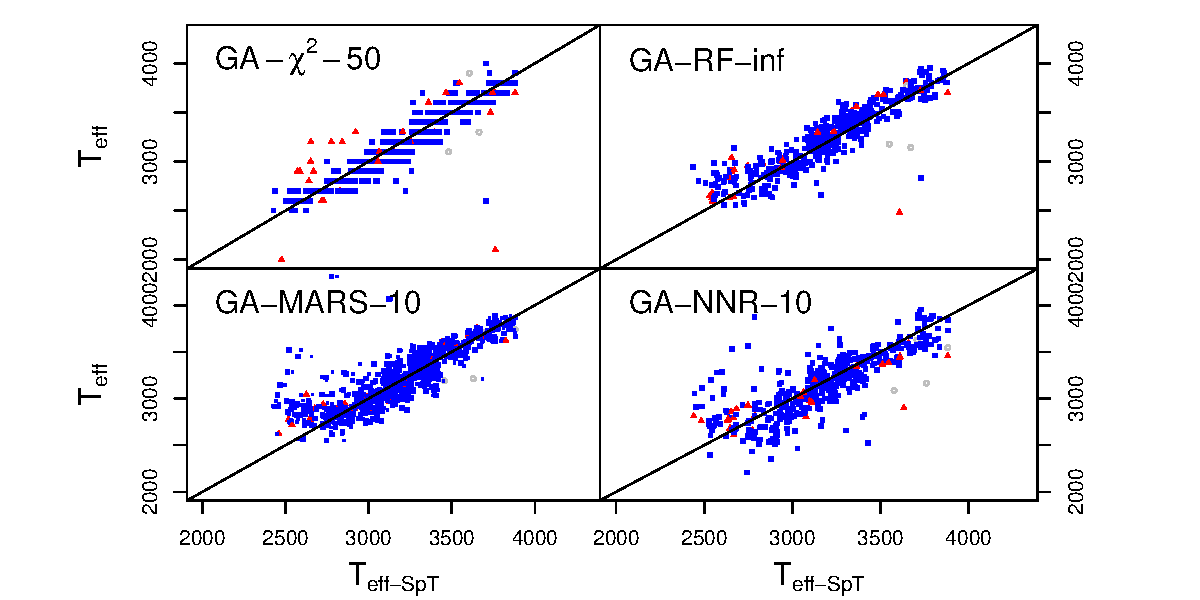
\includegraphics[width=\textwidth]{figs/ipac-teff}
\caption{Comparison
 between the effective temperatures derived from the tabulated
 spectral types in \protect\cite{cesetti} ($x$ axis) and those
 inferred by the various regression modules ($y$ axis): $\chi^2$
 module (top left, SNR=50), Random Forest Regression module (top
 right, SNR=$\infty$), GA-MARS module (bottom left, SNR=10), and the
 Neural Network module (bottom right, SNR=10).  Blue squares denote
 Main Sequence dwarfs and red triangles denote giant stars (luminosity
 class III) according to \protect\cite{cesetti}} \label{fig:ipac_teff}
\end {figure*}

Having shown that the feature selection with GAs degrades the
performance of regression models, one can wonder whether a different
feature selection procedure would produce better results. In
particular, we investigate the possibility that the features proposed
by \cite{cesetti} result in a performance equal to or even better than
the one achieved with $\chi^2$.

We train the same types of regression models to the features selected
in \cite{cesetti}, again learning from BT-Settl spectra of various
SNRs and predicting over the Dwarf Archives set. A summary of the results can be
found in Table \ref{tab:ipac-teff-rmse-cesetti}, where we use CS- to
indicate that the model was trained using the features
by \cite{cesetti}. 

For SNR=10, the best GA models (GA-KPLS in RMDSE or GA-RF in RMSE)
outperform the best CS model (GA-GBM). For SNR=50 the situation
depends on the figure-of-merit used to compare the regression models:
in RMSE the best model is CS-GBM while in RMDSE GA-GBM outperforms all
CS-models. Finally, for the unrealistic case of noiseless spectra,
Table \ref{tab:ipac-teff-rmse-cesetti} shows an overwhelming
degradation of the prediction accuracy from CS- features. But even in
the only case where the CS features outperform those selected by the
GA, the performance is below the one achieved by the minimum-$\chi^2$
approach. It is important to remark here that the features selected
in \cite{cesetti} were fit for the IRTF wavelength range and
resolution, and not all of them can be extracted from Dwarf Archives 
spectra. Hence, unlike in the case of the IRTF spectra, the comparison
of GA- and CS-based performances with Dwarf Archives spectra is not fair and the
results are only included for the sake of completeness.

The relationship between the GA predicted effective temperature and
the one measured by \cite{RA2012} (blue for the predictions by the
GA-MARS SNR=10 model and black for GA-RF SNR=$\infty$ model), and
by \cite{esm1} and \cite{esm2} (orange and green for
the same models as before) can be found in
Figure~\ref{fig:ipac_lt_lt}.

\begin{figure}
 \begin{center} \includegraphics[width=8cm]{figs/ipac_LG_Trojas_Tknn_10}

\caption{Relationship  between $\log(T_{\rm eff})$ from \protect\cite{RA2012}
in the $x$ axis and $\log(T_{\rm eff})$ as predicted by the GA-RF
 model with SNR=$\infty$ (black symbols, squares for dwarfs and a
 triangle for the only giant in the sample) and the GA-MARS trained
 with SNR=10 data (blue symbols). Green and orange symbols correspond
 to sources in common with \protect\cite{esm1}
 and \protect\cite{esm2} and the predictions by the
 GA-RF (SNR=$\infty$) and GA-MARS (SNR=10) models
 respectively.} \label{fig:ipac_lt_lt} \end{center}
\end{figure}



\subsubsection{Surface gravity models}

As in the IRTF exercise, we attempt to select features for surface
gravity estimation from BT-Settl spectra using GAs despite the much
lower spectral resolution and smaller wavelength coverage of the Dwarf Archives
spectra. Since there is no substantive compilation of surface
gravities that we could cross match with the IPAC list of M stars in
the Dwarf Archive, we are left with the same plausibility arguments
used in the IRTF study which are based on the $\log(T_{\rm
eff})$--$\log(g)$ diagram.

We again use the effective temperatures as input of the regression
models. Table~\ref{tab:ipac-logg-rmse} shows the cross-validation RMSE
and RMDSE for the same set of regression models used throughout this
article. It shows that the GA-RF model outperforms all other in all
SNR regimes, giving a consistent RMDSE of 1.0 dex. Obviously, this is
barely enough for classification in luminosity classes. Furthermore,
and as has been the case in the evaluation of all previous regression
modules, the cross-validation errors are poor estimates of the true
performances on real observed spectra. Figure \ref{fig:teffvsloggIPAC}
shows the $\log(T_{\rm eff})$--$\log(g)$ diagram for the best two
performing $\log(g)$ regression models (GA-NNR and GA-SVR, both
trained with SNR=10 BT-Settl spectra) and the two reference modules
based on the minimization of the $\chi^2$ (SNR=50) and the PPR-ICA
(SNR=10). Three of the four panels (all except the $\chi^2$
predictions) show a strong spurious correlation in the gravities of
the M dwarfs in the sense that the coolest dwarfs have unreasonable
values of $\log(g)$ around 2 dex. The PPR-ICA model shows this trend
too, but with a much shallower slope ($\log(g)\approx 4$ at
$\log(T_{\rm eff})\approx 3.4$). Only the GA-NNR module (and to a
lesser extent the $\chi^2$ module) places giant stars (red triangles)
in the locus expected judging by the values in Table 3
of \cite{cesetti} (black filled symbols) and the predictions for the
IRTF data set (green filled symbols). The various symbols (squares,
triangles, circles) reflect the luminosity classes found in either
Table 3 of \cite{cesetti} (for the IRTF values) or the DwarfArchives
table. 


\begin{figure*}
 \begin{center}
 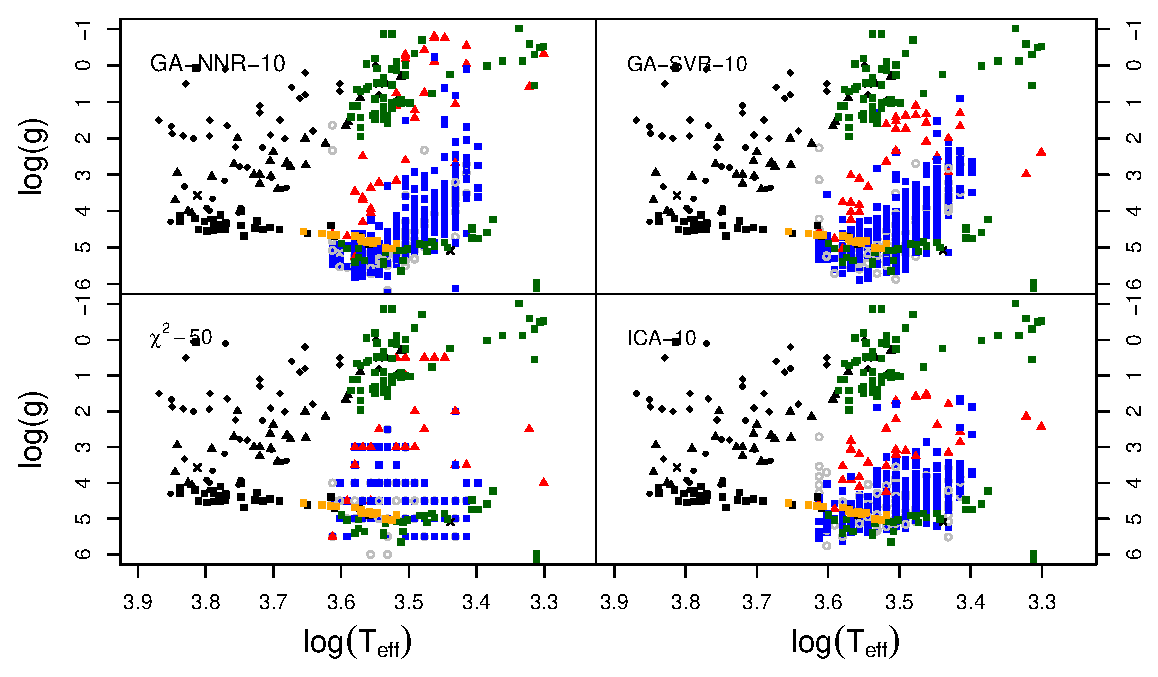
\includegraphics[width=\textwidth]{figs/ipac-teff-logg}

\caption{$\log(T_{\rm eff})$-$\log(g)$ planes obtained using the $\chi^2$ (SNR=50)
$\log(T_{\rm eff})$ preditions and the $\log(g)$ values from the
GA-NNR (SNR=10, top left), GA-SVR (SNR=10, top right), $\chi^2$
(SNR=50, bottom left), and PPR-ICA (SNR=10, bottom right) regression
models. Black symbols correspond to objects with physical parameters
in Table 3 of \protect\cite{cesetti}; green symbols correspond to the
predictions shown in Section \ref{sect:irtf-teff} for the IRTF
spectra; blue squares correspond to predictions for dwarf stars
according to the DwarfArchives.org luminosity classes; red triangles
correspond to giant stars according to DwarfArchives.org; orange
symbols correspond to values derived from high-resolution infrared
spectra by \protect\cite{esm1} and \protect\cite{esm2};
and finally, empty grey circles correspond to sources with no
luminosity class in DwarfArchives.org.}

\label{fig:teffvsloggIPAC}
 \end{center}
\end{figure*}

\subsubsection{Metallicity models} 

Finally, the same analysis is performed for metallicities, again using
the previously inferred temperature as a fixed input feature.
Table~\ref{tab:ipac-met-rmse} shows a summary of the cross-validation
performance of the different models.

In general, models trained with SNR=$\infty$ show much poorer
performace except for the GA-RF and GA-GBM cases. The best $\chi^2$
model produces errors almost a factor two larger than the
$GA-RF-\infty$ model (although it has to be borne in mind that, while
our regression models are capable of predicting metallicities that are
intermediate in the grid, the minimum $\chi^2$ can only yield values
in the grid, which has a step size of 0.5 dex). Models trained with
SNR=10 and 50, on the contrary, show a more consistent behaviour for
the entire set of regressors, with poorer performances than the
apparently optimal $GA-RF-\infty$, but also smaller differences
between models.

In order to select the best model, we again compare our model
predictions with the reference catalogs used in
Sect. \ref{sect:irtf-met}. We select the Random Forest trained with
noiseless synthetic spectra as the best model, which renders the
minimum RMSE (0.3 dex). Figure \ref{fig:ipac_mt} shows the comparison
of our estimates with the reference catalogs, using the same symbols
and colours as in Fig. \ref{MIRTF_ICA_10}.

Our value of the RMSE contrasts with the differences between estimates
for the same star in the literature. We obtain a mean difference of
0.1 dex a factor 3 smaller than our RMSE. 

\begin{figure}
 \begin{center} \includegraphics[width=8cm]{figs/ipac-figs/M-RFInf}

\caption{Relationship
 between the $RF-\infty$ predictions for metallicity and values from
 the literature for stars in the Dwarf Archives.  Black symbols
 represent values from \protect\cite{cesetti} ; orange symbols, values
 from \protect\cite{NevesIII}; green symbols, values that the Vizier
 catalog entry for Table 8 of \protect\cite{NevesIII} links
 to \protect\cite{Jao}, although we find no evidence
 that \protect\cite{Jao} contains estimates of metallicities; cyan and
 blue symbols, the values of [M/H] and [Fe/H] respectively
 in \protect\cite{RA2012}; red symbols, values
 from \protect\cite{Mann2015}; yellow symbols, values
 from \protect\cite{Newton2014}; and, finally, black symbols, values
 from \protect\cite{Gaidos2015}.}  \label{fig:ipac_mt} \end{center}
\end{figure}


It is interesting to note that our predictions extend to metallicities
as low as [M/H]=-2.1. Figure \ref{fig:ipac-hist-mets} shows a histogram of
the metallicities predicted by the GA-RF-$\infty$ model for the Dwarf Archives 
set of spectra. We find predictions below -1.5 for eleven sources, 6
of which have been previously identified as subdwarfs of different
categories (see Table \ref{tab:known-sds}).

\begin{figure}
	\begin{center}
		\includegraphics[width=8cm]{figs/ipac-figs/ipac-M-hist}

	\end{center}
        
        \caption{\label{fig:ipac-hist-mets}
Predictions of the GA-RF-$\infty$ regression model
        for the metallicity of Dwarf Archives stars.}

\end{figure}


\begin{table}\centering
	\begin{tabular}{@{}llll@{}}
		\hline
		Identifier & classification & Reference & GA-RF-$\infty$\\
		\hline
		LHS 3768 & usdM3 & \cite{1995AJ....109..797K}  & -2.1 \\
		LHS 2352 & esd   & \cite{1995AJ....109..797K}  & -2.0 \\
		LHS 1691 & usdM2 & \cite{0004-637X-669-2-1235} & -1.95\\
		LHS 2023 & esdM6 & \cite{0004-637X-672-2-1153} & -1.95\\
		LHS 515  & esdM5 & \cite{1538-3873-117-833-676}& -1.8\\
		LP471-17 & sdM   & \cite{1995AJ....109..797K}  & -1.7\\
		\hline
	\end{tabular}
        
	\caption{Previously known subdwarfs in the Dwarf Archives collection of
	spectra and the corresponding GA-RF-$\infty$ predictions.}

\label{tab:known-sds} 
\end{table}

The remaining 5 stars with metallicities below -1.5 are 2MASS
J17275631-3240430 (-2.0 dex); LHS 1625 (-1.97 dex); 2MASS
J19215188+2802275 (-1.9 dex); 2MASS J19004675+2806462 (-1.7 dex),
classified as K7III by \cite{1994ApJS...94..749K}); and 2MASS
J14465233-5320580 (-1.7 dex).



\section{Summary and conclusions}
\label{sec:summary}


{\bf TODO n: Write Summary \& Conclusions}


\section*{Acknowledgements}
This research has benefitted from the M, L, T, and Y dwarf compendium
of spectra housed at DwarfArchives.org.  The authors would like to
acknowledge funding by the Spanish Ministry of Economy and Innovation
through the grant AyA2014-55216. The IRTF library is provided by the
University of Hawaii under Cooperative Agreement no. NNX-08AE38A with
the National Aeronautics and Space Administration, Science Mission
Directorate, Planetary Astronomy Program. This research has made
extensive use of the R software \cite{R} and the {\it caret} R
package. Finally, 
the authors acknowledge the computer resources and technical assistance 
provided by the Centro de Supercomputaci\'on y Visualizaci\'on de Madrid (CeSViMa).

%-------------------------------------------------------------------


\begin{appendix}
\label{app}

\section{IRTF features}
\label{app:features:irtf}


\begin{table*}
\begin{center}

  \begin{tabular}{rrrr | rrrr | rrrr }
  \hline
 \multicolumn{4}{c}{SNR = $\infty$ } & \multicolumn{4}{c}{SNR = 10} &  \multicolumn{4}{c}{SNR=50} \\
  \hline
$\lambda_1$ & $\lambda_2$ & $\lambda_{cont;1}$ & $\lambda_{cont;2} $ & $\lambda_1$ & $\lambda_2$ & $\lambda_{cont;1}$ & $\lambda_{cont;2} $ & $\lambda_1$ & $\lambda_2$ & $\lambda_{cont;1}$ & $\lambda_{cont;2} $ \\ 
  \hline
9225.86  & 9283.94   & 9736.02  & 9793.96  & 8235.96  & 8294.04   & 12681.62 & 12768.68   &  8145.92 & 8204.03   & 12636.48 & 12723.57 \\   
11106.48 & 11193.56  & 13497.81 & 13613.95 & 8505.89  & 8563.93   & 13378.12 & 13494.13   &  8895.95 & 8953.95   & 11331.57 & 11418.65 \\     
13438.08 & 13554.08  & 12006.54 & 12093.56 & 9376.07  & 9433.92   & 12951.62 & 13038.62   &  8176.03 & 8234.13   & 10611.36 & 10698.46 \\      
9135.89  & 9193.91   & 10002.04 & 9999.92  & 8145.92  & 8204.03   & 12366.32 & 12453.33   &  13438.08 & 13554.08 & 12546.46 & 12633.49 \\     
9555.93  & 9614.06   & 12951.62 & 13038.62 & 9195.86  & 9253.93   & 9135.89 & 9193.92     &  8235.96 & 8294.04   & 11961.44 & 12048.54 \\      
9466.08  & 9523.82   & 13137.94 & 13253.96 & 9585.95  & 9644.12   & 10002.04 & 9999.92    &  9376.07 & 9433.92   & 10002.04 & 9999.92  \\   
11196.56 & 11283.24  & 12546.46 & 12633.49 & 8385.99  & 8443.94   & 11826.48 & 11913.28   &  9406.09 & 9463.96   & 13258.32 & 13374.32 \\    
8566.08  & 8624.07   & 13258.32 & 13374.32 & 9135.89  & 9193.92   & 9225.86 & 9283.94     &  9346.13 & 9403.92   & 13086.46 & 13194.09 \\   
8266.11  & 8324.03   & 9856.06  & 9913.91  & 13618.20 & 13734.15  & 11376.63 & 11463.51   &  11106.48 & 11193.56 & 13438.08 & 13554.08 \\    
8235.96  & 8294.04   & 12366.32 & 12453.33 & 9105.87  & 9163.91   & 8865.98 & 8923.94     &  9255.86 & 9314.01   & 8865.98  & 8923.94  \\    
\hline
\end{tabular}
\caption {Recommended features and continuum bandpasses for predicting
  $ T_{eff} $ using BT\_Settl with SNR= $ \infty ,  10 $ and $50$ and the IRTF
  wavelength range and resolution.} \label{tab:irtf-teff-noisy}
\end{center}
\end{table*}


\begin{table*}
\begin{center}
\begin{tabular}{rrrr | rrrr | rrrr}
  \hline
 \multicolumn{4}{c}{SNR =$ \infty$ } & \multicolumn{4}{c}{SNR = 10} &  \multicolumn{4}{c}{SNR=50} \\
  \hline
$\lambda_1$ & $\lambda_2$ & $\lambda_{cont;1}$ & $\lambda_{cont;2} $ & $\lambda_1$ & $\lambda_2$ & $\lambda_{cont;1}$ & $\lambda_{cont;2} $ & $\lambda_1$ & $\lambda_2$ & $\lambda_{cont;1}$ & $\lambda_{cont;2} $ \\ 
  \hline
     10245.88 & 10304.02 &	11241.29 & 11328.54 & 8176.03  & 8234.13  &	9165.87  & 9223.91  &  11151.63 & 11238.46 &      13086.46 & 13194.09 \\
     8415.91  & 8473.96  &	11511.51 & 11598.51 & 10485.99 & 10563.41 &	10002.04 & 9999.92  &  8385.99  & 8443.94  &      13618.20 & 13734.14 \\
     12906.56 & 12993.61 &	13041.48 & 13133.82 & 8656.09  & 8714.047 &      10926.46 & 11013.60 &  8176.03  & 8234.13  &      11241.29 & 11328.54 \\
     8716.00  & 8773.99  &	10425.90 & 10484.13 & 9525.89  & 9584.059 &	10002.04 & 9999.92  &  8536.03  & 8594.06  &      13041.48 & 13133.82 \\ 
     8805.93  & 8863.97  &	12816.72 & 12903.73 & 8205.98  & 8263.967 &	13041.48 & 13133.82 &  12771.70 & 12858.73 &      10306.03 & 10363.88 \\
     10126.02 & 10183.93 &	13086.46 & 13194.09 & 10275.97 & 10333.96 &	11376.63 & 11463.51 &  13378.12 & 13494.13 &      10002.04 & 9999.92  \\
     8176.03  & 8234.13  &	10971.57 & 11058.46 & 10306.03 & 10363.88 &	11151.63 & 11238.46 &  8626.02  & 8683.99  &      10926.46 & 11013.60 \\
     8626.02  & 8683.99  &	10746.43 & 10833.57 & 9165.87  & 9223.91  &	8385.99  & 8443.94  &  9826.05  & 9883.91  &      10006.07 & 10064.01 \\
     8536.03  & 8594.06  &	10215.95 & 10274.10 & 9645.82  & 9704.16  &	13137.94 & 13253.96 &  10521.56 & 10608.46 &      11736.71 & 11823.49 \\
     12951.62 & 13038.62 &	11196.56 & 11283.24 & 8326.00  & 8383.94  &	12726.69 & 12813.71 &  8205.98  & 8263.96  &      9796.09  & 9853.94  \\ 
   \hline
\end{tabular}
\caption {Recommended features and continuum bandpasses for predicting
  $log(g)$ using BT-Settl spectra of SNR= $\infty $ , $10$ and $50$ in the IRTF
  wavelength range and resolution.} \label{tab:irtf-logg-noisy}
\end{center}
\end{table*}


\begin{table*}
\begin{center}
\begin{tabular}{ rrrr | rrrr | rrrr }
  \hline
  \multicolumn{4}{c}{SNR = $\infty$ } & \multicolumn{4}{c}{SNR = 10} &  \multicolumn{4}{c}{SNR=50} \\
  \hline
$\lambda_1$ & $\lambda_2$ & $\lambda_{cont;1}$ & $\lambda_{cont;2} $ & $\lambda_1$ & $\lambda_2$ & $\lambda_{cont;1}$ & $\lambda_{cont;2} $ & $\lambda_1$ & $\lambda_2$ & $\lambda_{cont;1}$ & $\lambda_{cont;2} $ \\ 
  \hline

     12096.68 & 12183.66  & 12051.50 & 12096.68 & 8235.96  & 8294.04  &	11331.57 & 11418.65 & 9255.86 & 9314.01   &     13197.94 & 13313.92  \\
    9525.89 & 9584.05 	  & 12321.33 & 12408.32 & 9376.07  & 9433.92  &	10566.33 & 10653.62 & 8385.99 & 8443.94   &     9376.07  & 9433.92    \\
     8205.98 & 8263.96 	  & 10126.02 & 10183.93 & 10306.03 & 10363.88 &	 9942.14 & 9999.92  & 8716.00 & 8773.99   &     9585.95  & 9644.12    \\
     8566.08 & 8624.07 	  & 12276.52 & 12363.34 & 11286.42 & 11373.45 &	11241.29 & 11286.42 & 8235.96 & 8294.04   &     13086.46 & 13194.09  \\
     11196.56 & 11283.24  & 11151.63 & 11196.56 & 9676.00  & 9734.02  &	13086.46 & 13194.09 & 9676.00 & 9734.02   &     10791.44 & 10878.40  \\
     11151.639 & 11238.46 & 11466.35 & 11553.33 & 8775.95  & 8833.94  &	8415.91  & 8473.96  & 8415.91 & 8473.96   &     12411.34 & 12498.41  \\
     9555.93 & 9614.06 	  & 8205.98  & 8263.96  & 12411.34 & 12498.41 &	10245.88 & 10304.02 & 8446.03 & 8503.94   &     9406.09  & 9463.96    \\
     11016.62 & 11103.37  & 10791.44 & 10878.40 & 8476.01  & 8534.03  &	12276.52 & 12363.34 & 8205.98 & 8263.96   &     8955.88  & 9013.95    \\
     9766.16 & 9823.94 	  & 12681.62 & 12768.68 & 12636.48 & 12723.57 &	12051.50 & 12138.72 & 8985.93 & 9043.98   &     12186.62 & 12273.48  \\
     9942.14 & 9999.92    & 9555.93  & 9614.06  & 8415.91  & 8473.96  &	13618.20 & 13734.14 & 9015.98 & 9073.98   &     11241.29 & 11328.54  \\

\hline
\end{tabular}
\caption {Feature and Continuum bandpasses selected for predicting metallicity 
      using noisy BT\_Settl spectra with signal-to-noise ratios
      equal to $\infty , 10 $ and $ 50 $ in the IRTF wavelength range
  and resolution.} \label{tab:irtf-met-noisy}
\end{center}
\end{table*}


\section{Dwarf Archives features}
\label{app:features:ipac}


\begin{table*}
\begin{center}
\begin{tabular}{rrrr | rrrr | rrrr }
  \hline
 \multicolumn{4}{c}{SNR = $\infty $} &  \multicolumn{4}{c}{SNR = 10} &  \multicolumn{4}{c}{SNR=50} \\
  \hline
$\lambda_1$ & $\lambda_2$ & $\lambda_{cont;1}$ & $\lambda_{cont;2} $ & $\lambda_1$ & $\lambda_2$ & $\lambda_{cont;1}$ & $\lambda_{cont;2} $ & $\lambda_1$ & $\lambda_2$ & $\lambda_{cont;1}$ & $\lambda_{cont;2} $ \\ 
  \hline
7062 & 7094.4 &	7314 & 7346.4 & 7692 & 7724.4 &	6936 & 6968.4  & 7062 & 7094.4 &  7296 & 7328.4 \\
7116 & 7148.4 &	7782 & 7814.4 & 6990 & 7022.4 &	7998 & 8030.4  & 7026 & 7058.4 &  7044 & 7076.4 \\
7134 & 7166.4 &	7872 & 7904.4 & 6900 & 6932.4 &	7548 & 7580.4  & 7080 & 7112.4 &  7926 & 7958.4 \\
6900 & 6932.4 &	7764 & 7796.4 & 7854 & 7886.4 &	7710 & 7742.4  & 6900 & 6932.4 &  7548 & 7580.4 \\
7170 & 7202.4 &	7890 & 7922.4 & 7116 & 7148.4 &	7908 & 7940.4  & 7134 & 7166.4 &  7836 & 7868.4 \\
7080 & 7112.4 &	7926 & 7958.4 & 7278 & 7310.4 &	7926 & 7958.4  & 7296 & 7328.4 &  7962 & 7994.4 \\
7188 & 7220.4 &	7548 & 7580.4 & 7152 & 7184.4 &	7746 & 7778.4  & 6936 & 6968.4 &  7728 & 7760.4 \\
7800 & 7832.4 &	7962 & 7994.4 & 7134 & 7166.4 &	7764 & 7796.4  & 6972 & 7004.4 &  6900 & 6932.4 \\
6990 & 7022.4 &	7008 & 7040.4 & 6918 & 6950.4 &	6900 & 6932.4  & 6990 & 7022.4 &  7944 & 7976.4 \\
7026 & 7058.4 &	6990 & 7022.4 & 7224 & 7256.4 &	7962 & 7994.4  & 6918 & 6950.4 &  7782 & 7814.4 \\

\hline
\end{tabular}
\caption {Spectral features and continuum bandpasses selected by the
  GA for predicting $ T_{eff}$ using BT\_Settl spectra with SNR= $\infty ,10 $ and
  $ 50 $ in the Dwarf Archives wavelength range and
  resolution.} \label{tab:ipac-teff-noisy}
\end{center}
\end{table*}


\begin{table*}
\begin{center}
\begin{tabular}{rrrr | rrrr | rrrr}
  \hline
 \multicolumn{4}{c}{SNR = $\infty $} & \multicolumn{4}{c}{SNR = 10} &  \multicolumn{4}{c}{SNR=50} \\
  \hline
$\lambda_1$ & $\lambda_2$ & $\lambda_{cont;1}$ & $\lambda_{cont;2} $ & $\lambda_1$ & $\lambda_2$ & $\lambda_{cont;1}$ & $\lambda_{cont;2} $ & $\lambda_1$ & $\lambda_2$ & $\lambda_{cont;1}$ & $\lambda_{cont;2} $ \\ 
  \hline
7134 & 7166.4 &	7044 & 7076.4 & 6990 & 7022.4 &	6918 & 6950.4 & 6918 & 6950.4 & 6936 & 6968.4  \\
6954 & 6986.4 &	7152 & 7184.4 & 6900 & 6932.4 &	7278 & 7310.4 & 6936 & 6968.4 & 7836 & 7868.4  \\
7512 & 7544.4 &	7890 & 7922.4 & 7062 & 7094.4 &	7242 & 7274.4 & 7656 & 7688.4 & 7890 & 7922.4  \\
7062 & 7094.4 &	7224 & 7256.4 & 7692 & 7724.4 &	7008 & 7040.4 & 6900 & 6932.4 & 7872 & 7904.4  \\
6936 & 6968.4 &	7854 & 7886.4 & 7656 & 7688.4 &	7998 & 8030.4 & 7008 & 7040.4 & 7044 & 7076.4  \\
6900 & 6932.4 &	7746 & 7778.4 & 6936 & 6968.4 &	7836 & 7868.4 & 7512 & 7544.4 & 7656 & 7688.4  \\
6918 & 6950.4 &	7800 & 7832.4 & 7206 & 7238.4 &	7062 & 7094.4 & 7440 & 7472.4 & 7332 & 7364.4  \\
7008 & 7040.4 &	7134 & 7166.4 & 7512 & 7544.4 &	7926 & 7958.4 & 7800 & 7832.4 & 7692 & 7724.4  \\
7872 & 7904.4 &	7008 & 7040.4 & 7764 & 7796.4 &	7710 & 7742.4 & 7404 & 7436.4 & 7548 & 7580.4  \\
7962 & 7994.4 &	7980 & 8012.4 & 7404 & 7436.4 &	7548 & 7580.4 & 7080 & 7112.4 & 7152 & 7184.4  \\
   \hline
\end{tabular}
\caption {Spectral features and continuum bandpasses selected by the
  GA for predicting $\log(g)$ using BT\_Settl spectra of SNR= $\infty , 10 $ and $ 50 $
  in the Dwarf Archives wavelength range and
  resolution.} \label{tab:ipac-logg-noisy}
\end{center}
\end{table*}


\begin{table*}
\begin{center}
\begin{tabular}{rrrr | rrrr | rrrr }
  \hline
 \multicolumn{4}{c}{SNR = $\infty $} & \multicolumn{4}{c}{SNR = 10} &  \multicolumn{4}{c}{SNR=50} \\
  \hline
$\lambda_1$ & $\lambda_2$ & $\lambda_{cont;1}$ & $\lambda_{cont;2} $ & $\lambda_1$ & $\lambda_2$ & $\lambda_{cont;1}$ & $\lambda_{cont;2} $ & $\lambda_1$ & $\lambda_2$ & $\lambda_{cont;1}$ & $\lambda_{cont;2} $ \\ 
  \hline
7188 & 7220.4 &	7854 & 7886.4 & 7692 & 7724.4 &	7026 & 7058.4  &  7098 & 7130.4 & 7926 & 7958.4 \\
7080 & 7112.4 &	7926 & 7958.4 & 6900 & 6932.4 &	7008 & 7040.4  &  7188 & 7220.4 & 7962 & 7994.4  \\
7116 & 7148.4 &	7098 & 7130.4 & 7350 & 7382.4 &	7908 & 7940.4  &  7368 & 7400.4 & 7980 & 8012.4  \\
7422 & 7454.4 &	7836 & 7868.4 & 6918 & 6950.4 &	6900 & 6932.4  &  7116 & 7148.4 & 7872 & 7904.4  \\
7350 & 7382.4 &	7998 & 8030.4 & 7098 & 7130.4 &	7314 & 7346.4  &  7062 & 7094.4 & 7206 & 7238.4  \\
7224 & 7256.4 &	7818 & 7850.4 & 7440 & 7472.4 &	7872 & 7904.4  &  7584 & 7616.4 & 7170 & 7202.4  \\
7710 & 7742.4 &	7062 & 7094.4 & 7134 & 7166.4 &	7962 & 7994.4  &  6936 & 6968.4 & 6918 & 6950.4  \\
7476 & 7508.4 &	7944 & 7976.4 & 7368 & 7400.4 &	7926 & 7958.4  &  7692 & 7724.4 & 7890 & 7922.4  \\
7134 & 7166.4 &	7584 & 7616.4 & 7080 & 7112.4 &	7044 & 7076.4  &  7134 & 7166.4 & 7548 & 7580.4  \\
7836 & 7868.4 &	7278 & 7310.4 & 7044 & 7076.4 &	7980 & 8012.4  &  7494 & 7526.4 & 7998 & 8030.4  \\
\hline
\end{tabular}
\caption {Spectral features and continuum bandpasses selected by the
  GA for predicting metallicities using BT\_Settl spectra of SNR= $\infty , 10 $
  and $ 50 $ in the Dwarf Archives wavelength range and
  resolution.} \label{tab:ipac-met-noisy}
\end{center}
\end{table*}


\begin{appendix}
\label{app:rmse}
\section{IRTF RMSE regression models}

\newcommand{\ra}[1]{\renewcommand{\arraystretch}{#1}}
\begin{table*}\centering
\ra{1.3}
\begin{tabular}{@{}lrrcrrcrr@{}}\toprule
& \multicolumn{2}{c}{$SNR = 10$} & \phantom{ab}& \multicolumn{2}{c}{$SNR = 50$} &
\phantom{ab} & \multicolumn{2}{c}{$SNR = \infty$}\\
\cmidrule{2-3} \cmidrule{5-6} \cmidrule{8-9}
$Regression Models$ & $RMSE$ & $RMDSE$ && $RMSE$ & $RMDSE$ && $RMSE$ & $RMDSE$ \\ \midrule
$\chi^2$      & 232      & \bf{100}&& 235      & 120    && 232      & \bf{100} \\
 PPR-ICA      & 242      & 128        && 242      &  99    && 280      & 162 \\
 GA-RF        & 308      & 183        && 248      & 136    && \bf{167} & 135 \\
 GA-GBM       & 287      & 160        && 248      & 149    && 233      & 113 \\
 GA-SVR       & \bf{221} & 122        && 281      & 151    && 299      & 160 \\
 GA-NNET      & 283      & 192        && 264      & 114    && 326      & 212 \\
 GA-KNN       & 238      & 120        && \bf{232} & 137    && 219      & \bf{100}  \\
 GA-MARS      & 253      & 113        && 254      & \bf{95}&& 226      & 133 \\
 GA-KPLS      & 275      & 120        && 300      & 119    && 387      & 218 \\
\bottomrule
\end{tabular}
\caption {Cross-validation RMSE and RMDSE for the various regression
  models that predict $T_{eff}$ (K) in the IRTF wavelength range and
  resolution.}
\label{tab:irtf-teff-rmse} 
% \end{center}
\end{table*}


\begin{table*}\centering
\ra{1.3}
\begin{tabular}{@{}lrrr@{}}\toprule
& {$SNR = 10$} & {$SNR = 50$} & {$SNR = \infty$}\\ \midrule
$\chi^2 $            &  -77 &  -87  & -85 \\
$ICA+ppr$            & -104 & -55   & -130 \\
GA-RR                & -102 &  -39  & 170 \\
GA-RF                & -173 & -127  &  -5 \\
GA-GBM               & -141 & -109  &  32 \\
GA-SVR               &  -58  &  -3  &  92 \\
GA-NNET              & -147 &  -36  &  39 \\
GA-KNN               &  -76  &-110  & -67 \\
GA-MARS              &  -57  & -88  &  98 \\
GA-KPLS              & -120 &   -4  & 214 \\
\bottomrule
\end{tabular}
\caption {Average bias in the $T_{eff}$ (K) estimates computed (IRTF
  wavelength range and resolution) with respect to the reference
  values in Table 3 of \cite{cesetti}.}
\label{irtf-teff-bias} 
% \end{center}
\end{table*}

\begin{table*}\centering
\ra{1.3}
\begin{tabular}{@{}rrrcrrcrr@{}}\toprule
& \multicolumn{2}{c}{$SNR = 10$} & \phantom{ab}& \multicolumn{2}{c}{$SNR = 50$} &
\phantom{ab} & \multicolumn{2}{c}{$SNR = \infty$}\\
\cmidrule{2-3} \cmidrule{5-6} \cmidrule{8-9}
$Regression Models$ & $RMSE$ & $RMDSE$ && $RMSE$ & $RMDSE$ && $RMSE$ & $RMDSE$ \\ \midrule
CS-RF               & 234       & 180       && {\bf 264} & 218       &&  {\bf 321} & 265 \\
CS-GBM              & {\bf 232} & 195       && 268       & 254       &&  325       & 246 \\
CS-SVR              & 268       & 227       && 293       & 257       &&  432       & 364 \\
CS-NNET             & 357       & 255       && 357       & {\bf 204} &&  552       & 435 \\
CS-KNN              & 249       & 172       && 293       & 256       &&  327       & {\bf 230}\\
CS-KPLS             & 351       & {\bf 162} && 856       & 456       && 1086       & 535 \\
\hline
\end{tabular}
\caption {Regression model performance based on the features proposed
  by \cite{cesetti}}
\label{irtf-teff-rmse-cesetti}
%\end{center}
\end{table*}


\ra{1.3}
\begin{table*}\centering
\begin{tabular}{@{}rrrcrrcrr@{}}\toprule
& \multicolumn{2}{c}{$SNR = 10$} & \phantom{ab}& \multicolumn{2}{c}{$SNR = 50$} &
\phantom{ab} & \multicolumn{2}{c}{$SNR = \infty$}\\
\cmidrule{2-3} \cmidrule{5-6} \cmidrule{8-9}
$Regression Models$ & $RMSE$ & $RMDSE$ && $RMSE$ & $RMDSE$     && $RMSE$       & $RMDSE$ \\ \midrule
$\chi^2$          & 0.82       & 0.45      && 0.93       & 0.61       && 3.5        & 3.48 \\
$ PPR-ICA$        & 0.54       & 0.48      && {\bf 0.3}  & {\bf 0.17} && 0.72       & 0.57 \\
GA-RF             & 0.64       & \bf{0.38} && 0.77       & 0.72       && 0.53       & 0.39 \\
GA-GBM            & {\bf 0.48} & 0.45      && 0.61       & 0.47       && 0.49       & 0.41 \\
GA-SVR            & 0.66       & 0.40      && 0.63       & 0.58       && {\bf 0.46} & \bf{0.21} \\
GA-NNET           & 0.78       & 0.61      && 0.47       & 0.44       && 1.2        & 0.97 \\
GA-MARS           & 0.84       & 0.57      && 0.54       & 0.37       && 0.99       & 0.76 \\
GA-KNN            & 1.23       & 0.83      && 1.39       & 1.44       && 1.60       & 1.32 \\
GA-KPLS           & 0.99       & 0.99      && 0.51       & 0.49       && 0.96       & 0.77 \\
GA-RR             & 0.74       & 0.57      && 0.50       & 0.47       && 0.57       & 0.41 \\

\bottomrule
\end{tabular}
\caption {RMSE and RMDSE for the various $\log(g)$ regression models
  [dex] in the IRTF wavelength range and resolution.}
\label{tab:irtf-logg-rmse} 
% \end{center}
\end{table*}

\ra{1.3}
\begin{table*}\centering
\begin{tabular}{@{}rrrcrrcrr@{}}\toprule
& \multicolumn{2}{c}{$SNR = 10$} & \phantom{ab}& \multicolumn{2}{c}{$SNR = 50$} &
\phantom{ab} & \multicolumn{2}{c}{$SNR = \infty$}\\
\cmidrule{2-3} \cmidrule{5-6} \cmidrule{8-9}
$Regression Models$ & $RMSE$ & $RMDSE$ && $RMSE$ & $RMDSE$     && $RMSE$       & $RMDSE$ \\ \midrule
$\chi^2$    & 0.76 & 0.22      && 0.36 & 0.18     && 0.36 & 0.18 \\
$PPR-ICA$   & 0.24 & \bf{0.13} && 0.31 & 0.22     && 0.43 & 0.27 \\
$GA-RF$     & 0.33 & 0.25      && 0.73 & 0.41     && 0.61 & 0.36 \\
$GA-GBM$    & 0.27 & 0.19      && 0.70 & 0.52     && 0.63 & 0.35 \\
$GA-SVR$    & 0.33 & 0.22      && 0.45 & 0.32     && 0.92 & 0.89 \\
$GA-NNET$   & 0.37 & 0.30      && 0.33 & 0.37     && 0.95 & 0.81 \\
$GA-KNN$    & 0.69 & 0.55      && 0.23 & \bf{0.15}&& 0.21 & \bf{0.15} \\ 
$GA-MARS$   & 0.36 & 0.16      && 0.49 & 0.41     && 0.83 & 0.85 \\
$GA-RR$     & 0.31 & 0.17      && 0.30 & 0.24     && 0.78 & 0.23 \\

\bottomrule
\end{tabular}
\caption {RMSE and RMDSE for the various regression models (IRTF
  wavelength range and resolution) predicting metallicity [dex].}
\label{tab:irtf-met-rmse} 
% \end{center}
\end{table*}


\section{IPAC RMSE regression models}

% According to Joaqu. this is with respect to the spectral types
% 
\begin{table*}\centering
\ra{1.3}
\begin{tabular}{@{}rrrcrrcrr@{}}\toprule
& \multicolumn{2}{c}{$SNR = 10$} & \phantom{ab}& \multicolumn{2}{c}{$SNR = 50$} &
\phantom{ab} & \multicolumn{2}{c}{$SNR = \infty$}\\
\cmidrule{2-3} \cmidrule{5-6} \cmidrule{8-9}
$Regression Models$ & $RMSE$ & $RMDSE$ && $RMSE$ & $RMDSE$ && $RMSE$ & $RMDSE$ \\ \midrule
$\chi^2$    & {\bf 147} & 79       && {\bf 121} & {\bf 56}  && {\bf 126} & {\bf 57} \\
$ PPR-ICA$  & 188       & 126      && 164       & 95        && 191       & 130 \\
GA-RF       & 160       & 97       && 196       & 103       && 145       & 94 \\
GA-GBM      & 175       & 105      && 225       & 99        && 185       & 94 \\
GA-SVR      & 203       & 112      && 285       & 106       && 368       & 154 \\
GA-NNET     & 221       & 84       && 313       & 111       && 395       & 202 \\
GA-KNN      & 183       & 119      && 193       & 109       && 224       & 110  \\
GA-MARS     & 222       & 76       && 361       & 103       && 374       & 157 \\
GA-KPLS     & 227       & {\bf 72} && 331       & 123       && 409       & 208 \\
\bottomrule
\end{tabular}
\caption {RMSE and RMDSE for the various regression models that predict $T_{eff}$ (K) in the IPAC wavelength range and resolution.} 
\label{tab:ipac-teff-rmse} 
% \end{center}
\end{table*}

\begin{table*}
\begin{center}
\begin{tabular}{@{}rrrcrrcrr@{}}\toprule
& \multicolumn{2}{c}{$SNR = 10$} & \phantom{ab}& \multicolumn{2}{c}{$SNR = 50$} &
\phantom{ab} & \multicolumn{2}{c}{$SNR = \infty$}\\
\cmidrule{2-3} \cmidrule{5-6} \cmidrule{8-9}
$Regression Models$ & $RMSE$ & $RMDSE$ && $RMSE$ & $RMDSE$     && $RMSE$       & $RMDSE$ \\ \midrule
CS-RF   & 203       & 140       && 243       & {\bf 121} &&  {\bf 306} &  {\bf 172}  \\
CS-GBM  & {\bf 188} & {\bf 120} && {\bf 161} & 138       &&  337       &  222  \\
CS-SVR  & 197       & 135       && 379       & 194       &&  840       &  688  \\
CS-NNET & 207       & 135       && 514       & 296       &&  719       &  489  \\
CS-MARS & 252       & 124       && 789       & 186       && 3464       &  784  \\
CS-KNN  & 235       & 158       && 246       & 137       &&  314       &  175  \\
CS-KPLS & 250       & 201       && 741       & 361       && 2247       & 1424  \\
CS-RR   & 211       & 128       && 400       & 239       &&  828       &  774  \\

\hline
\end{tabular}
\caption {Performances of regression models trained on the features
  selected by \cite{cesetti} and applied to BT-Settl spectra in the IPAC wavelength range and resolution.}
\label{tab:ipac-teff-rmse-cesetti}
\end{center}
\end{table*}

% HERE 2: This must be wrong: the Chi^2 and ICA columns are almost empty
% so I have asked Joaquín why. If the RMDSE are computed from these empty columns, these figures are just wrong.
% Answer: Wrong RData
% REDO tables and discussion

\ra{1.3}
\begin{table*}\centering
\begin{tabular}{@{}rrrcrrcrr@{}}\toprule
& \multicolumn{2}{c}{$SNR = 10$} & \phantom{ab}& \multicolumn{2}{c}{$SNR = 50$} &
\phantom{ab} & \multicolumn{2}{c}{$SNR = \infty$}\\
\cmidrule{2-3} \cmidrule{5-6} \cmidrule{8-9}
$Regression Models$ & $RMSE$ & $RMDSE$ && $RMSE$ & $RMDSE$     && $RMSE$       & $RMDSE$ \\ \midrule
$\chi^2$    & 2.2       & 1.6       && 2.2       & 1.4       && 2.2       & 1.6 \\
PPR-ICA     & 2.1       & 1.8       && 1.8       & 1.4       && 4.3       & 4.2 \\
GA-RF       & {\bf 1.3} & {\bf 1.0} && {\bf 1.6} & {\bf 1.1} && {\bf 1.4} & {\bf 0.9} \\
GA-GBM      & 1.6       & 1.1       && 1.7       & 1.4       && 1.7       & 1.2 \\
GA-SVR      & 2.0       & 1.8       && 2.1       & 1.9       && 2.3       & 1.6 \\
GA-NNET     & 2.0       & 1.8       && 2.2       & 1.9       && 3.2       & 2.8 \\
GA-MARS     & 1.8       & 1.5       && 2.0       & 1.7       && 2.0       & 1.5 \\
GA-KNN      & 2.0       & 1.5       && 2.2       & 1.7       && 1.7       & 1.2 \\
GA-KPLS     & 1.8       & 1.4       && 2.0       & 1.7       && 2.7       & 2.3 \\
GA-RR       & 2.0       & 1.8       && 2.1       & 1.8       && 3.7       & 3.2 \\

\bottomrule
\end{tabular}
\caption {RMSE and RMDSE for the various regression models predicting $Log(G)$ [dex] in the IPAC wavelength range and resolution.} 
\label{tab:ipac-logg-rmse} 
% \end{center}
\end{table*}

\ra{1.3}
\begin{table*}\centering
\begin{tabular}{@{}rrrcrrcrr@{}}\toprule
& \multicolumn{2}{c}{$SNR = 10$} & \phantom{ab}& \multicolumn{2}{c}{$SNR = 50$} &
\phantom{ab} & \multicolumn{2}{c}{$SNR = \infty$}\\
\cmidrule{2-3} \cmidrule{5-6} \cmidrule{8-9}
$Regression Models$ & $RMSE$ & $RMDSE$ && $RMSE$ & $RMDSE$     && $RMSE$       & $RMDSE$ \\ \midrule
$\chi^2$    & 0.55 & 0.27 && 0.51 & 0.29 && 0.43  & 0.29 \\
$PPR-ICA$   & 0.48 & 0.27 && 0.70 & 0.39 && 0.85  & 0.71 \\
$GA-RF$     & 0.55 & 0.38 && 0.71 & 0.61 && 0.23  & 0.16 \\
$GA-GBM$    & 0.64 & 0.43 && 0.87 & 0.84 && 0.31  & 0.23 \\
$GA-SVR$    & 0.46 & 0.26 && 0.57 & 0.44 && 3.38  & 2.33 \\
$GA-NNET$   & 0.52 & 0.45 && 0.66 & 0.54 && 2.03  & 1.88 \\
$GA-KNN$    & 0.37 & 0.28 && 0.99 & 0.78 && 0.56  & 0.32 \\ 
$GA-MARS$   & 0.71 & 0.47 && 0.80 & 0.69 && 1.15  & 0.68 \\
%$ pls $    & 0.67  & 0.61  && 0.63  & 0.55 && 1.17 & 1.02 \\ 
$GA-RR$     & 0.47 & 0.29 && 0.50 & 0.36 && 1.18  & 1.18 \\

\bottomrule
\end{tabular}
\caption {RMSE and RMDSE for the various regression models predicting $Met$ [dex] in the IPAC wavelength range and resolution.} 
\label{tab:ipac-met-rmse} 
% \end{center}
\end{table*}


  \end{appendix}


\begin{appendix}
\label{app:figures}
  \section{Results with features from \cite{cesetti}}
\label{app:figures:irtf}


\begin {figure*}
 \centering
  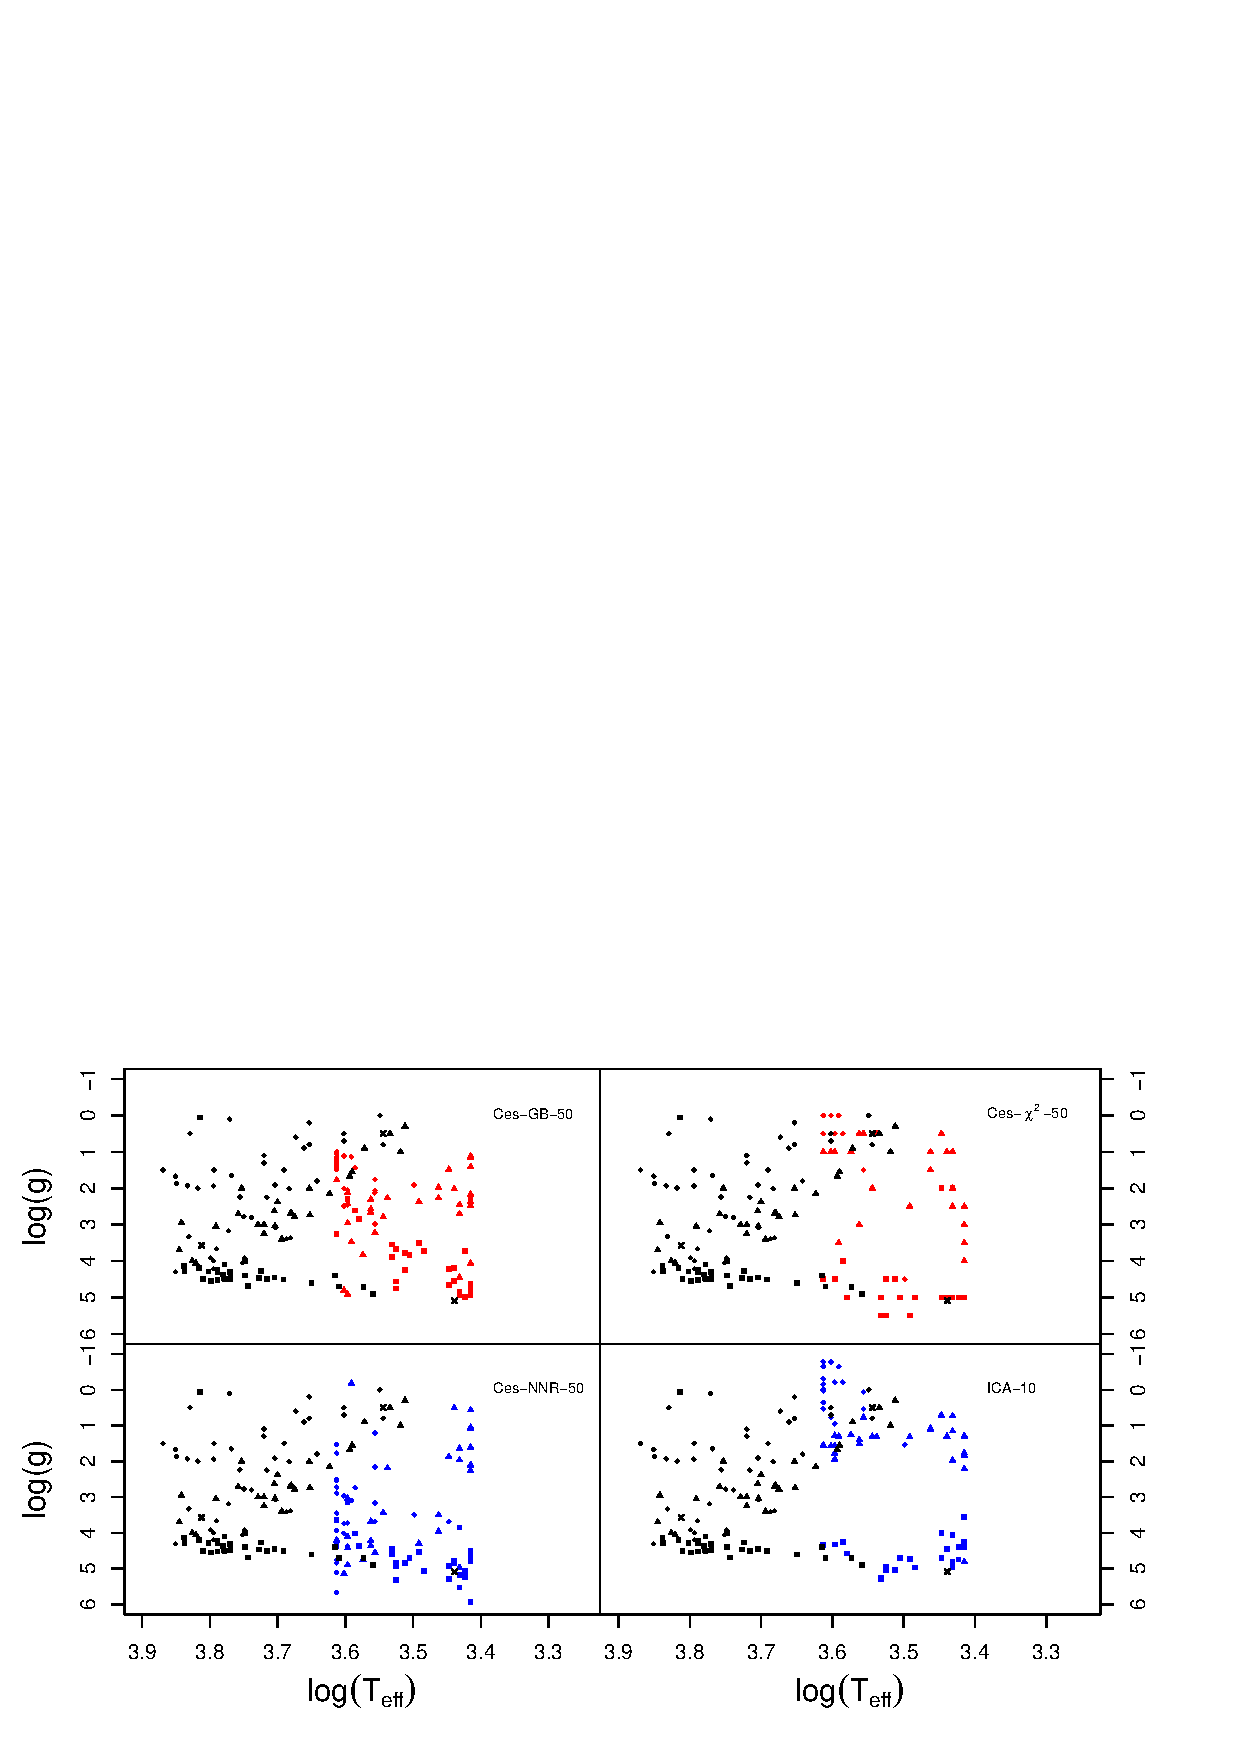
\includegraphics[width=\textwidth]{figs/irtf-figs/irtf-Cesseti.pdf}
  \caption{$\log(T_{eff})$--$\log(g)$ diagrams produced by the CES-KNN
    (SNR=$\infty$) effective temperatures, and gravities derived with
    the CES-GB (SNR=50), CES-$\chi^2$ (SNR=50), CES-NNR (SNR=50), and $ICA-10$
    models (clockwise, starting from the top left plot).}
 \label{fig:irtf-ces}
\end {figure*}



\begin {figure}
\centering
\includegraphics[width=0.45\textwidth]{figs/irtf-figs/M-CES.pdf}
\caption{Comparison of the CES-RF (SNR=50) regression model
  predictions with the estimates of the metallicity in the
  literature. The symbols and colours are the same as in Figure
  \ref{MIRTF_ICA_10}.}
\label{fig:irtf-ces-met}
\end {figure}


\begin {figure*}
 \centering
  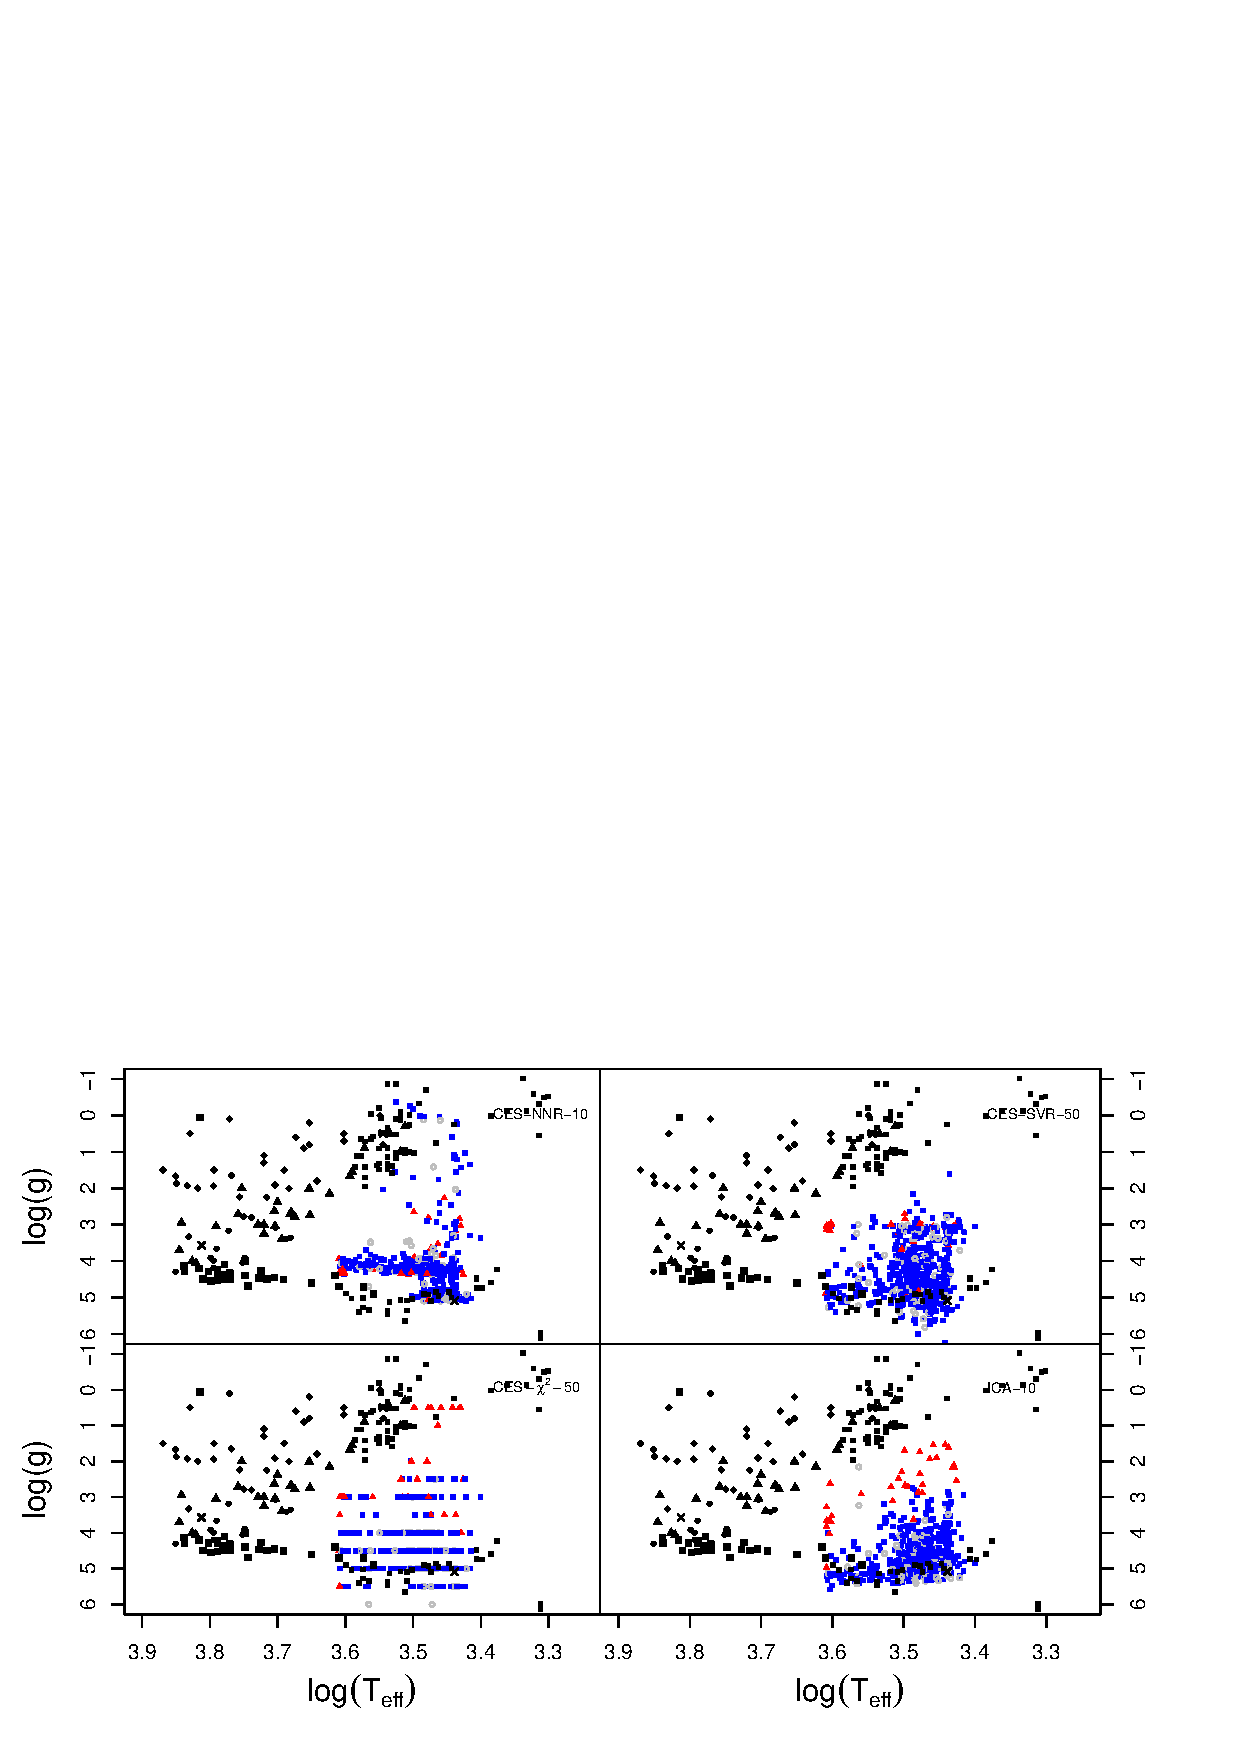
\includegraphics[width=\textwidth]{figs/ipac-Cesseti.pdf}
  \caption{}
 \label{fig:ipac-ces}
\end {figure*}



\end{appendix}

\end{appendix}


\bibliography{references_m}{}
\bibliographystyle{mnras}

\end{document}
